\documentclass{report}

\usepackage{lmodern}
\renewcommand*\familydefault{\sfdefault}
\usepackage[T1]{fontenc}
\usepackage[utf8]{inputenc}
\usepackage[francais]{babel}
\usepackage[nottoc,numbib]{tocbibind}

\usepackage[colorlinks,pagebackref]{hyperref}
\usepackage{amsmath}
\usepackage{amsfonts}
\usepackage{stmaryrd}
\usepackage{xcolor}
\definecolor{lightgray}{rgb}{.9,.9,.9}
\usepackage{graphicx}
\usepackage[justification=centering]{caption}
\usepackage{placeins}
\usepackage{listings}
\usepackage{tikz}
\usetikzlibrary{positioning,shapes,arrows,automata,petri}
\usetikzlibrary{intersections}

% TODO UPMC, Bérard, Roux, ...
\title{Rapport de stage \\
  {\bf Robustesse des modèles temporisés : \\
    une étude de cas}}
\author{Armel Mangean}
\date{Septembre 2014}

\begin{document}

  \pagenumbering{alph}
  \maketitle

  \pagenumbering{arabic}
  \chapter*{Remerciement}

    Je tiens à remercier dans un premier temps toute l'équipe pédagogique de
    l'Université Pierre et Marie Curie et tous les intervenants responsables de
    la formation du Master Informatique fillière Système et Application
    Réparties pour avoir assuré la qualité d'enseignement de celle-ci. Je
    remercie plus particulièrement madame Béatrice Bérard pour avoir assuré le
    rôle de maitre de stage.

    ~

    Je tiens à remercier et à témoigner ma reconnaissance aux personnes
    suivantes pour l'experience enrichissante que j'ai pu vivre durant c'est 5
    mois à l'IRCCyN et l'École Centrale Nantes. Messieurs Olivier H. Roux,
    Jean-Luc Béchennec, Sébastien Faucou, Didier Lime et Richard Urunela pour
    leur confiance, le temps qu'ils ont pu me consacrer tout au long de cette
    période et pour avoir toujours répondu à mes interrogations.

    ~

    Je remercie également Benjamin Sientzoff avec qui j'ai colaboré ainsi que
    nombreux doctorants et stagiaires de l'IRCCyN pour leur accueil sympathique
    ainsi que pour leur aide. Enfin je remercie ma famille et mes amis qui m'ont
    sontenu durant ce stage.

  \tableofcontents

  \chapter*{Introduction}
  \addcontentsline{toc}{chapter}{Introduction}

    C'est avec enthousiasme que j'effectue ma dernière année de Master
    Informatique en Systèmes et Applications Réparties au sein de l'Université
    Pierre et Marie Curie. Dans le cadre de ma cinquième année d'étude dans
    l'enseignement supérieur, je réalise un stage de fin de Master au sein de
    l'Institut de Recherche en Communication et Cybernétique de Nantes,
    l'IRCCyN.

    ~
    
    Ce stage me donne les moyens de mettre en pratique l'ensemble de mes
    connaissances et compétences dans un cadre professionnel. La tâche qui m'est
    confiée est la modélisation et la vérification d'un ensemble de propriétés
    d'un robot devant servir à un démonstrateur dans le cadre de différents
    projets de recherches.

    ~

    Le sujet initial de ce stage était la génération d'applicatifs temps réel à
    partir de modèles formels. Cependant, certaines contraintes s'étant
    présentées plus ou moins tôt dans la réalisation de ce stage et certains
    choix réalisés en conséquent ont fait se réorienter mes axes de travail. Le
    travail réalisé constitue finalement une étude de cas sur la robustesse des
    modèles temporisés. Cette étude porte sur une sous-partie du démonstrateur.

    ~

    Pour rendre la lecture de ce document accessible au plus grand nombre je me
    suis efforcé d'expliquer les concepts techniques de manière le plus simple
    possible. Dans un premier temps, je developperai le contexte de
    réalisation de ce stage. Dans un second temps, j'aborderai les missions qui
    m'ont été confiées et le travail réalisé en conséquent. Enfin, je décrirai
    les résultats obtenus et le bilan qui peut en être fait.
    
  \chapter{Contexte}
  \section{Scolaire}
    
    Ce stage s'inscrit dans mon cursus scolaire en tant que stage de fin
    d'étude. J'arrive effectivement à la fin du Master que j'ai eu la chance de
    réaliser à l'Université Pierre et Marie Curie. J'y ai effectué un Master
    Informatique dans la filière Systèmes et Applications Réparties. En fin de
    seconde année j'ai opté pour l'option Systèmes Répartis Embarqués et Temps
    Réel. C'est dans cette voie que s'inscrit mon stage puisqu'il se situe dans
    le domaine du temps réel embarqué.

    ~
    
    Ce stage a une orientation recherche au sens où il requiert une étude de
    divers travaux de l'état de l'art dans la modèlisation des systèmes temps
    réel. Il s'inscrit dans un projet de recherche académique et a pour objet
    la mise en \oe uvre de résultats de recherches théoriques.

    ~
    
    Ce stage m'ouvre la porte vers le monde de la recherche où j'aimerais
    entamer ma carrière professionnelle. Ce stage est en effet la dernière étape
    dans le projet scolaire qui a été le mien depuis mon entrée en Institut
    Universitaire de Technologie en Informatique à Nantes. C'est alors que j'ai
    construit mon ambition de travailler dans la recherche publique et que j'ai
    rencontré les enseignants qui m'ont suivit jusqu'à ce jour dans mon
    parcours.
    
  \section{Professionnel}
    \subsection{L'IRCCyN}

      Il m'a été donné l'opportunité de réaliser mon stage à l'IRCCyN,
      l'Institut de Recherche en Communication et Cybernetique de Nantes. Cet
      établissement est une Unité Mixte de Recherche, du Centre National pour la
      Recherche Scientifique qui a pour ambition d'étendre l'ensemble des
      connaissances actuelles autour de ce qui concerne l'interaction entre les
      systèmes, la cybernétique.

      ~
    
      Cela représente un large champs d'étude et de nombreux domaines y sont
      donc étudiés. Parmis ces domaines on peut en autres trouver la logistique,
      la psychologie cognitive, la bioinformatique, l'automatique, le traitement
      du signal, la robotique, etc.
        
      ~
    
      Mon stage a débuté le 7 Avril 2014 et prendra fin le 12 Septembre
      2014. Une fermeture administrative de 2 semaine en début Août m'aura
      permis de profiter de cet été 2014.

    \subsection{L'équipe Systèmes Temps Réel}

      Au sein de cet ensemble de domaines d'étude se trouve l'informatique et
      plus précisement l'informatique temps réel. Elle définit des méthodes et
      techniques nécessaires à la mise en place de systèmes informatiques
      critiques. Ici, le terme critique dénote d'une part un besoin important
      en fiabilité, autrement dit il s'agit de systèmes ne devant pas
      défaillir, et d'autre part de certaines contraintes liées à un respect
      d'échéances temporelles.

      ~
    
      On peut prendre pour exemple le système informatique intégré aux voitures
      modernes permettant d'améliorer le confort de conduite et surtout la
      sécurité des passagers par un contrôle informatisé du véhicule. Cela est
      permis par l'identification des situations dangereuses et les réponses qui
      sont alors appliquées dans des délais brefs.

      ~
    
      Au fil des années ces sytèmes deviennent de plus en plus performants du
      point de vue de l'usager mais bien évidemment de plus en plus complexes du
      point de vue du concepteur, demandant donc toujours plus de travail pour
      les construire. C'est le rôle de l'équipe Systèmes Temps Réel de l'IRCCyN,
      au sein de laquelle j'effectue mon stage, de produire des outils
      facilitant la conception et l'analyse de tels systèmes.


  \chapter{Mission}
  \section{Projet}

      Ce rapport de stage constitue un livrable dans le cadre du projet
      ImpRo\footnotemark pour {\it Implementatbility and Robustness of Timed
        Systems}. Ce projet est financé par l'Agence Nationale de la Recherche
      dans le cadre du Programme Blanc. Il s’interesse aux problèmes liés aux
      implémentations des modèles formels des systèmes embarqués communicants.
      \footnotetext{\url{http ://anr-impro.irccyn.ec-nantes.fr}}

      ~
    
      Les différentes entitées universitaires collaborant à ce projet sont
      l'IRCCyN (Nantes), l'IRISA (Rennes), le LIP6, le LSV, le LIAFA (Paris) et
      le LIF (Marseille). Son coordinateur est Didier Lime de l'équipe Systèmes
      Temps Reél de l'IRCCyN.

      ~
      
      Ce projet adresse les problèmes liés aux mises en \oe uvre pratiques des
      modélisations formelles des systèmes embarqués communicants. Ces modèles
      abstraient beaucoup d’aspects complexes ou de limitations de leur
      environnement d’exécution. La modélisation du temps, en particulier, est
      habituellement idéale, avec des horloges infiniment précises, des tests ou
      des changements de mode instantanés. L’objectif de ce projet est d’étudier
      dans quelle mesure les implémentations de ces modèles préservent leurs
      propriétés.

      ~
    
      La robustesse d’un modèle caractérise l’amplitude de la différence
      existant entre ce modèle et une mise en \oe uvre qui en est faite. Cette
      difference réside, pour une part, dans l’écart entre la modèlisation d’un
      système et son implementation, pour une autre part, dans l’écart entre la
      modélisation de l’environement du système et l’environement réellement
      constaté. Si un écart faible ne permet pas de préserver les propriétés
      constatées sur le modèle alors celui-ci est considéré comme peu robuste.
      L'un des objectifs du projet est de mesurer et éventuellement réduire la
      distance qui existe entre un modèle d'un système et sa réalisation.

      ~
    
      Plusieurs approches d'analyse de robustesse des modèles temporisés ont été
      développées dans le cadre de ce projet. Dans ce rapport nous nous
      concentrons sur deux d'entre elles. La première approche s'appuie sur la
      réduction des automates temporisés, la seconde sur la synthèse de
      paramètres temporels.

      ~

      Afin de
      mettre en évidence les résultats théoriques issus de ce projet il a été
      proposé de réaliser un démonstrateur. Celui-ci est un système réel qui peut
      être modélisé et analysé à l'aide des outils mathématiques étudiés dans le
      projet. Une spécification du démontrateur a été réalisée \cite{bechennec12}.

    \subsection{Spécification}

      \begin{figure}
        \centering
        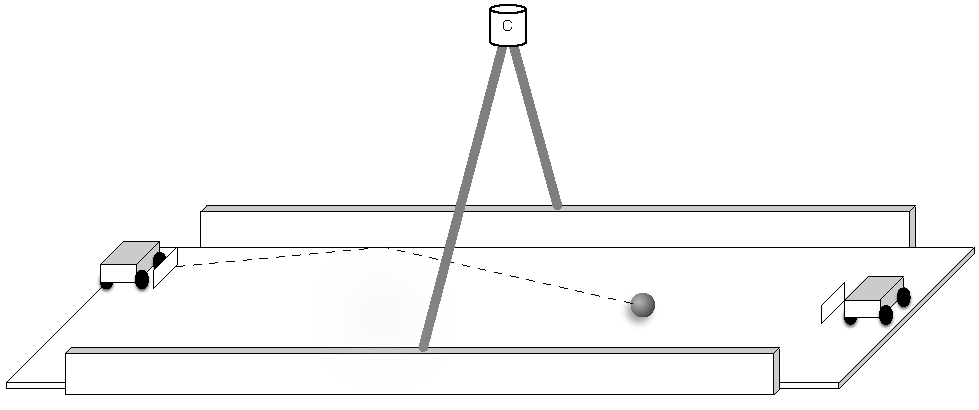
\includegraphics[width=0.8\textwidth]{./img/spec-demo1.pdf}
        \caption{Schéma de la spécification, vue isométrique}
        \label{fig:spec-demo1}
      \end{figure}

      \begin{figure}
        \centering
        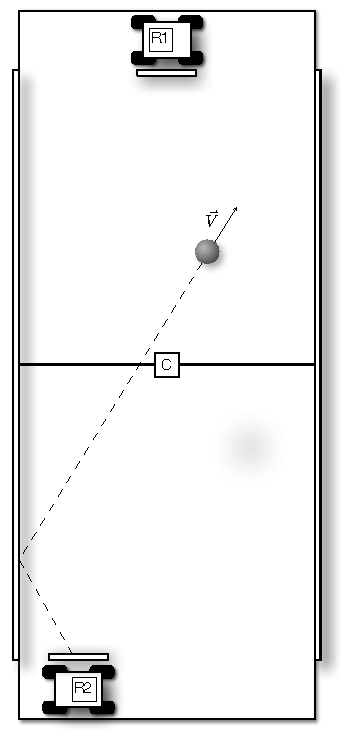
\includegraphics[angle=270, width=0.8\textwidth]{./img/spec-demo2.pdf}
        \caption{Schéma de la spécification, vue du dessus}
        \label{fig:spec-demo2}
      \end{figure}

      Le démonstrateur est un système de deux robots qui jouent à un jeu inspiré
      du {\it air kockey}. Dans ce jeu, chaque joueur cherche à faire sortir la
      balle du terrain par le côté du joueur adverse. Le terrain est représenté
      vu du dessus sur la figure \ref{fig:spec-demo1} et en perspective
      isométrique sur la figure \ref{fig:spec-demo2}. Le terrain est
      rectangulaire. Les longueurs sont équipées de rebords sur lesquels la
      balle vient rebondir. Les robots sont équipés d'un dispositif permettant
      de récupérer et de frapper la balle ainsi que de roues non
      directrices. Ils se déplacent dans le sens de la largeur du terrain, sur
      des rigoles.

      ~
    
      Les robots sont réalisés à l'aide du kit robotique Lego Mindstorms NXT. Le
      système d'exploitation temps réel Trampoline est utilisé pour exploiter
      les microcontrôleurs qui équipent ces kits. Ce système d'exploitation est
      un logiciel libre dont le développement est principalement assuré par
      l'équipe Systèmes Temps Réel de l'IRCCyN.

      ~
    
      Le logiciel de pilotage des robots est un logiciel temps réel. Des
      contraintes temps réel sont ainsi associées aux fonctions de pilotage des
      organes du robot (moteur qui entraîne les roues, moteurs de manipulation
      de la raquette), et aux fonctions de planification des déplacements
      (récupération de la trajectoire de la balle, positionnement en regard de
      la balle). Le système d'exploitation Trampoline offre les services
      nécessaires à la garantie de ces contraintes.
  
      ~
    
      Pour déterminer la position à atteindre pour pouvoir frapper la balle, les
      robots interrogent une station centrale qui fournit la position et
      l'accélération de la balle. Cette information est capturée à l'aide d'une
      caméra située au-dessus du terrain.

      \subsubsection{Modifications des spécifications}

        Par contrainte technique, certains éléments de cette spécification
        initiale ont été ajustés afin de garantir la faisabilité du
        démonstrateur. En effet, des essais préalables ont montré que les temps
        de latence des communications de la station centrale vers les robots
        cumulés aux temps de traitements sur la station centrale étaient trop
        important pour permettre la réalisation du démonstrateur.

        ~
    
        L'implémentation actuelle n'inclus pus de station centrale. Son rôle de
        détection de la balle a été remplacée par une caméra embarquée pouvant
        réaliser des traitements d'images simples. Cette caméra est associée à
        un Arduino Uno réalisant la communication avec le robot Lego via un bus
        I2C.

        ~
        
        La mise en \oe uvre de cette modification de la spéficiation du
        démonstrateur a donné lieu à un stage réalisé par Benjamin Sientzoff
        s'étant déroulé de Juin à Juillet 2014.

  \section{Besoin}

    Le travail attendu est la réalisation d'une étude de cas non-triviale sur
    la robustesse des modèles temporisés s'appuyant sur le démonstrateur issu
    du projet ImpRo. Ce travail s'articule en plusieurs volets : la
    modélisation du démonstrateur, l'implémentation du modèle réalisé et des
    vérifications formelles et pratique des propriétés du modèle.

    \subsection{Modélisation}

      Deux types de modélisations sont attendues. La première modélisation
      attendue est une modélisation architecturale du démonstrateur. Elle décrit
      l'architecture matérielle et logicielle du démonstrateur. Cette
      modélisation a pour principal objectif d'être un support de
      documentation sur l'arichitecture du démonstrateur. Elle doit permettre
      aux personnes travaillant sur d'autre aspect dans le cadre du projet
      Impro ou dans le cadre d'autres projets aux thématiques avoisinantes
      d'appréhender le fonctionnement du démonstrateur de manière simple.

      Un des rôles de cette modélisation est en conséquence d'introduire des
      noms qui pourront être retrouvés dans la seconde modélisation. Ces noms
      permettront de faire le lien entre les deux modélisations.

      ~
  
      La seconde modélisation attendue est une modèlisation comportementale du
      démontrateur. Elle définit le comportement de celui-ci. Ce sont les
      modèles issus de cette modélisation qui serviront de support aux
      différentes analyses et vérifications qui sont attendues. Un des rôles
      de cette modélisation est également de servir de support à
      l'implémentation des robots du démonstrateur.

    \subsection{Implémentation}

      Suite à certaines contraintes propre à l'équipe Système Temps Réel,
      l'implémentation matérielle du démonstrateur n'a pu être complétement
      réalisée avant le début de mon stage. Ce démonstrateur a vocation à être
      réutiliser dans le cadre d'autres projets de recherche. Il est donc
      attendu un travail soigné et documenté qui puisse être facilement
      réutiliser par d'autres personnes, stagiaires comme
      enseignants-chercheurs.

      ~

      Il m'est donc demandé de
      travailler à compléter ainsi qu'à modifier l'implémentation matérielle
      du démonstrateur. Celle-ci doit integrer un permier moteur pour le
      déplacement latéral, un second moteur pour la manipulation de la
      raquette permettant le tir, une caméra permettant de suivre la balle à
      distance, des capteurs de proximité permettant de repérer la balle à
      proximité et un capteur de distance permettant de définir le
      positionnement latéral du robot.

      ~
  
      L'implémentation logicielle doit assurer des propriétés temps réel. Elle
      sera donc réalisée grâce à un jeu de tâches qui sera ordonnancé par
      un système d'exploitation temps réel. Ces tâches doivent réalisées les
      fonctions liées à l'implémentation matérielle. C'est à dire commander le
      déplacement latéral du robot en fonction de la position de la balle et
      celle du robot ainsi qu'actionner la raquette afin de tirer dans la balle
      lorsque celle-ci se trouve à proximité.

    \subsection{Vérification}

      Les vérifications qui seront réalisées constitueront une mise en \oe
      uvre des résultats de recherche issu du projet Impro. Cette mise en \oe
      uvre prendra la forme de vérifications formelles sur des modèles
      temporisés. Les résultats de ces vérifications nous donnerons un
      indicateur quand à la robustesse des modèles considérés.

      ~
      
      Les propriétés que l'on souhaite vérifier sont en rapport avec la notion
      de robustesse des modèles. Ici, on souhaite montrer que telle ou telle
      sous-partie du modèle du système est robuste ou non-robuste. De même, on
      souhaite montrer que sous certaines contraintes liées à l'implémentation
      du modèle le système est faisable ou non en regard à un comportement
      attendu du démonstrateur. 

      Une fois les résultats théoriques sur la robustesse du démonstrateur
      obtenus, ceux-ci pourront être analysé et comparer aux constatations
      concrètes qui peuvent être fais sur le fonctionnement du démonstrateur.


  \chapter{Travaux}
  \section{Modélisation}
    \subsection{Modélisation architecturale}
      
      Afin de réaliser la modélisation architecturale c'est AADL\cite{aadl} qui a
      été choisi. AADL, pour {\it Architecture Analysis \& Design Language}, est
      un langage de modélisation d'architectures des sytèmes embarqués et temps
      réel issu de la recherche avionique. De fait, il ne définit pas qu'une
      syntaxe permettant de composer des modèles mais également une sémantique
      qui en fait un outil de modélisation spécifique au domaine de l'embarqué.

      ~

      AADL été conçu originellement en tant qu'un langage textuel. Le but d'une
      telle démarche était de garantir une complète definition de sa syntaxe. De
      fait, il est possible de réaliser des vérifications, des simulations et de
      générer du code source à partir de modèles AADL. Le standard AADL défini
      aujourd'hui trois format de modèles AADL. Un format textuel utile à la
      réalisation de modélisations complètes et détaillées. Un format graphique
      utile au processus de conception et à la documentation. Un format basé sur
      XML utile à l'exploitation des modèles AADL par des outils informatique.

    % TODO Mettre en avant ce qui se retrouve dans la modélisation comportementale
    \subsubsection{Première spécification}

      Il s'agit ici d'une modélisation architecturale basée sur la première
      version des spécifications du démonstrateur. Une modélisation s'appuyant
      sur la seconde version des spécifications sera présentée par la suite.
      
      ~
  
      \begin{figure}[!ht]
        \centering 
        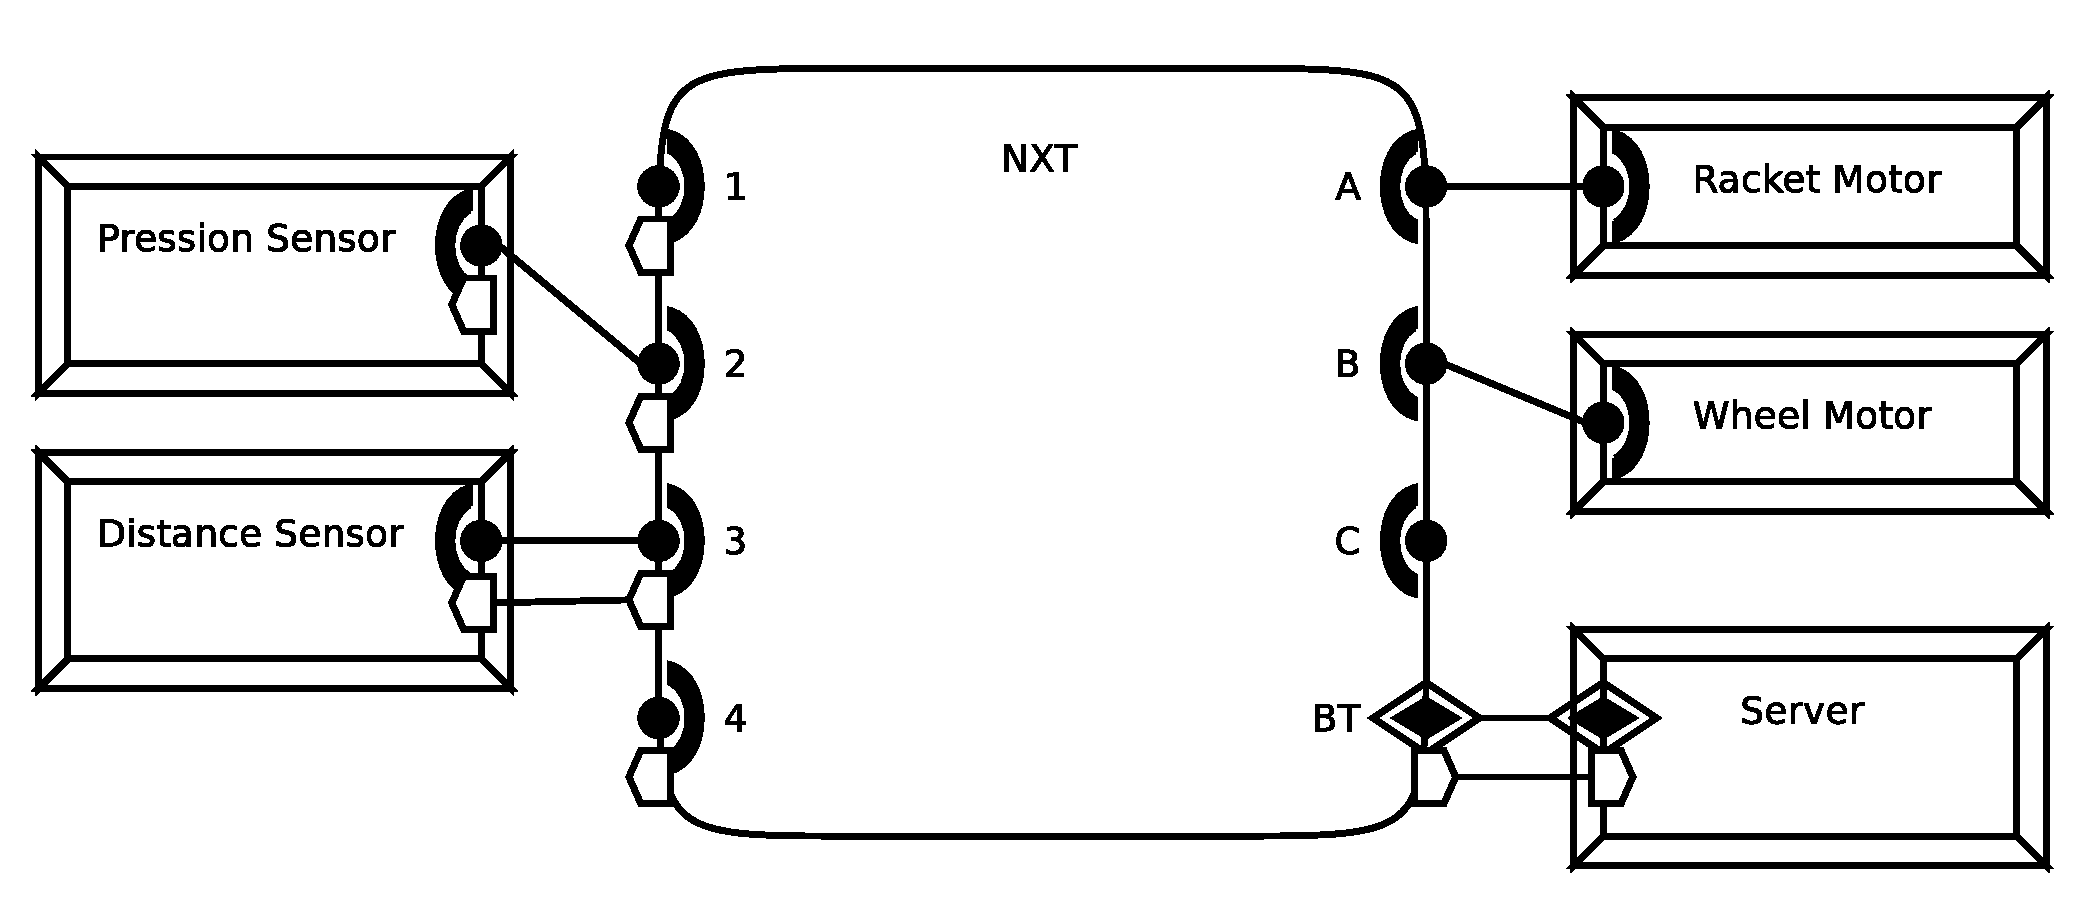
\includegraphics[scale=0.25]{./img/aadl-robot1.pdf}
        \caption{Vue global du système.}
        \label{fig:aadl-robot1}
      \end{figure}
        
      La figure \ref{fig:aadl-robot1} offre une représentation
      graphique du macro-modèle du robot. Le composant principal est
      le système {\it NXT}, les composants l'entourant sont des
      périphériques. Afin de réaliser son positionnement latéral le
      robot est équipé d'un capteur de distance ({\it Distance
        Sensor}), d'une connection à un serveur par {\it bluetooth}
      ({\it Server}) et d'un moteur actionnant une roue ({\it Wheel
        Motor}). Afin de frapper la balle le robot est équipé d'un
      moteur actionnant une raquette ({\it Racket Motor}) ainsi que
      d'un capteur de pression indiquant la fin de course de la
      raquette ({\it Pression Sensor}).

      Le système {\it NXT} est constitué de quatre groupes de ports
      d'entrées indexés de 1 à 4 et de trois groupes de ports de
      sorties indexés de A à C. À ceux-xi s'ajoute un port
      d'entrée/sortie inquiqué par le label BT.

      Le flux de données entre le capteur de pression et le système
      est réalisé par une connection d'entrée/sortie de type {\it digital I/O}.
      Les flux de données entre les deux moteurs et le systèmes sont
      réalisés par des connections à modulation largeur d'impulsion
      ({\it PWM}). Le flux de données et d'évènements entre le capteur
      de distance et le système est réalisé par une connexion sur
      un bus {\it I2C}. Enfin, le flux de données et d'évènements entre le
      serveur et le système est réalisé par une connexion sur un bus {\it
        bluetooth}.

      ~

      \begin{figure}[!ht]
        \centering
        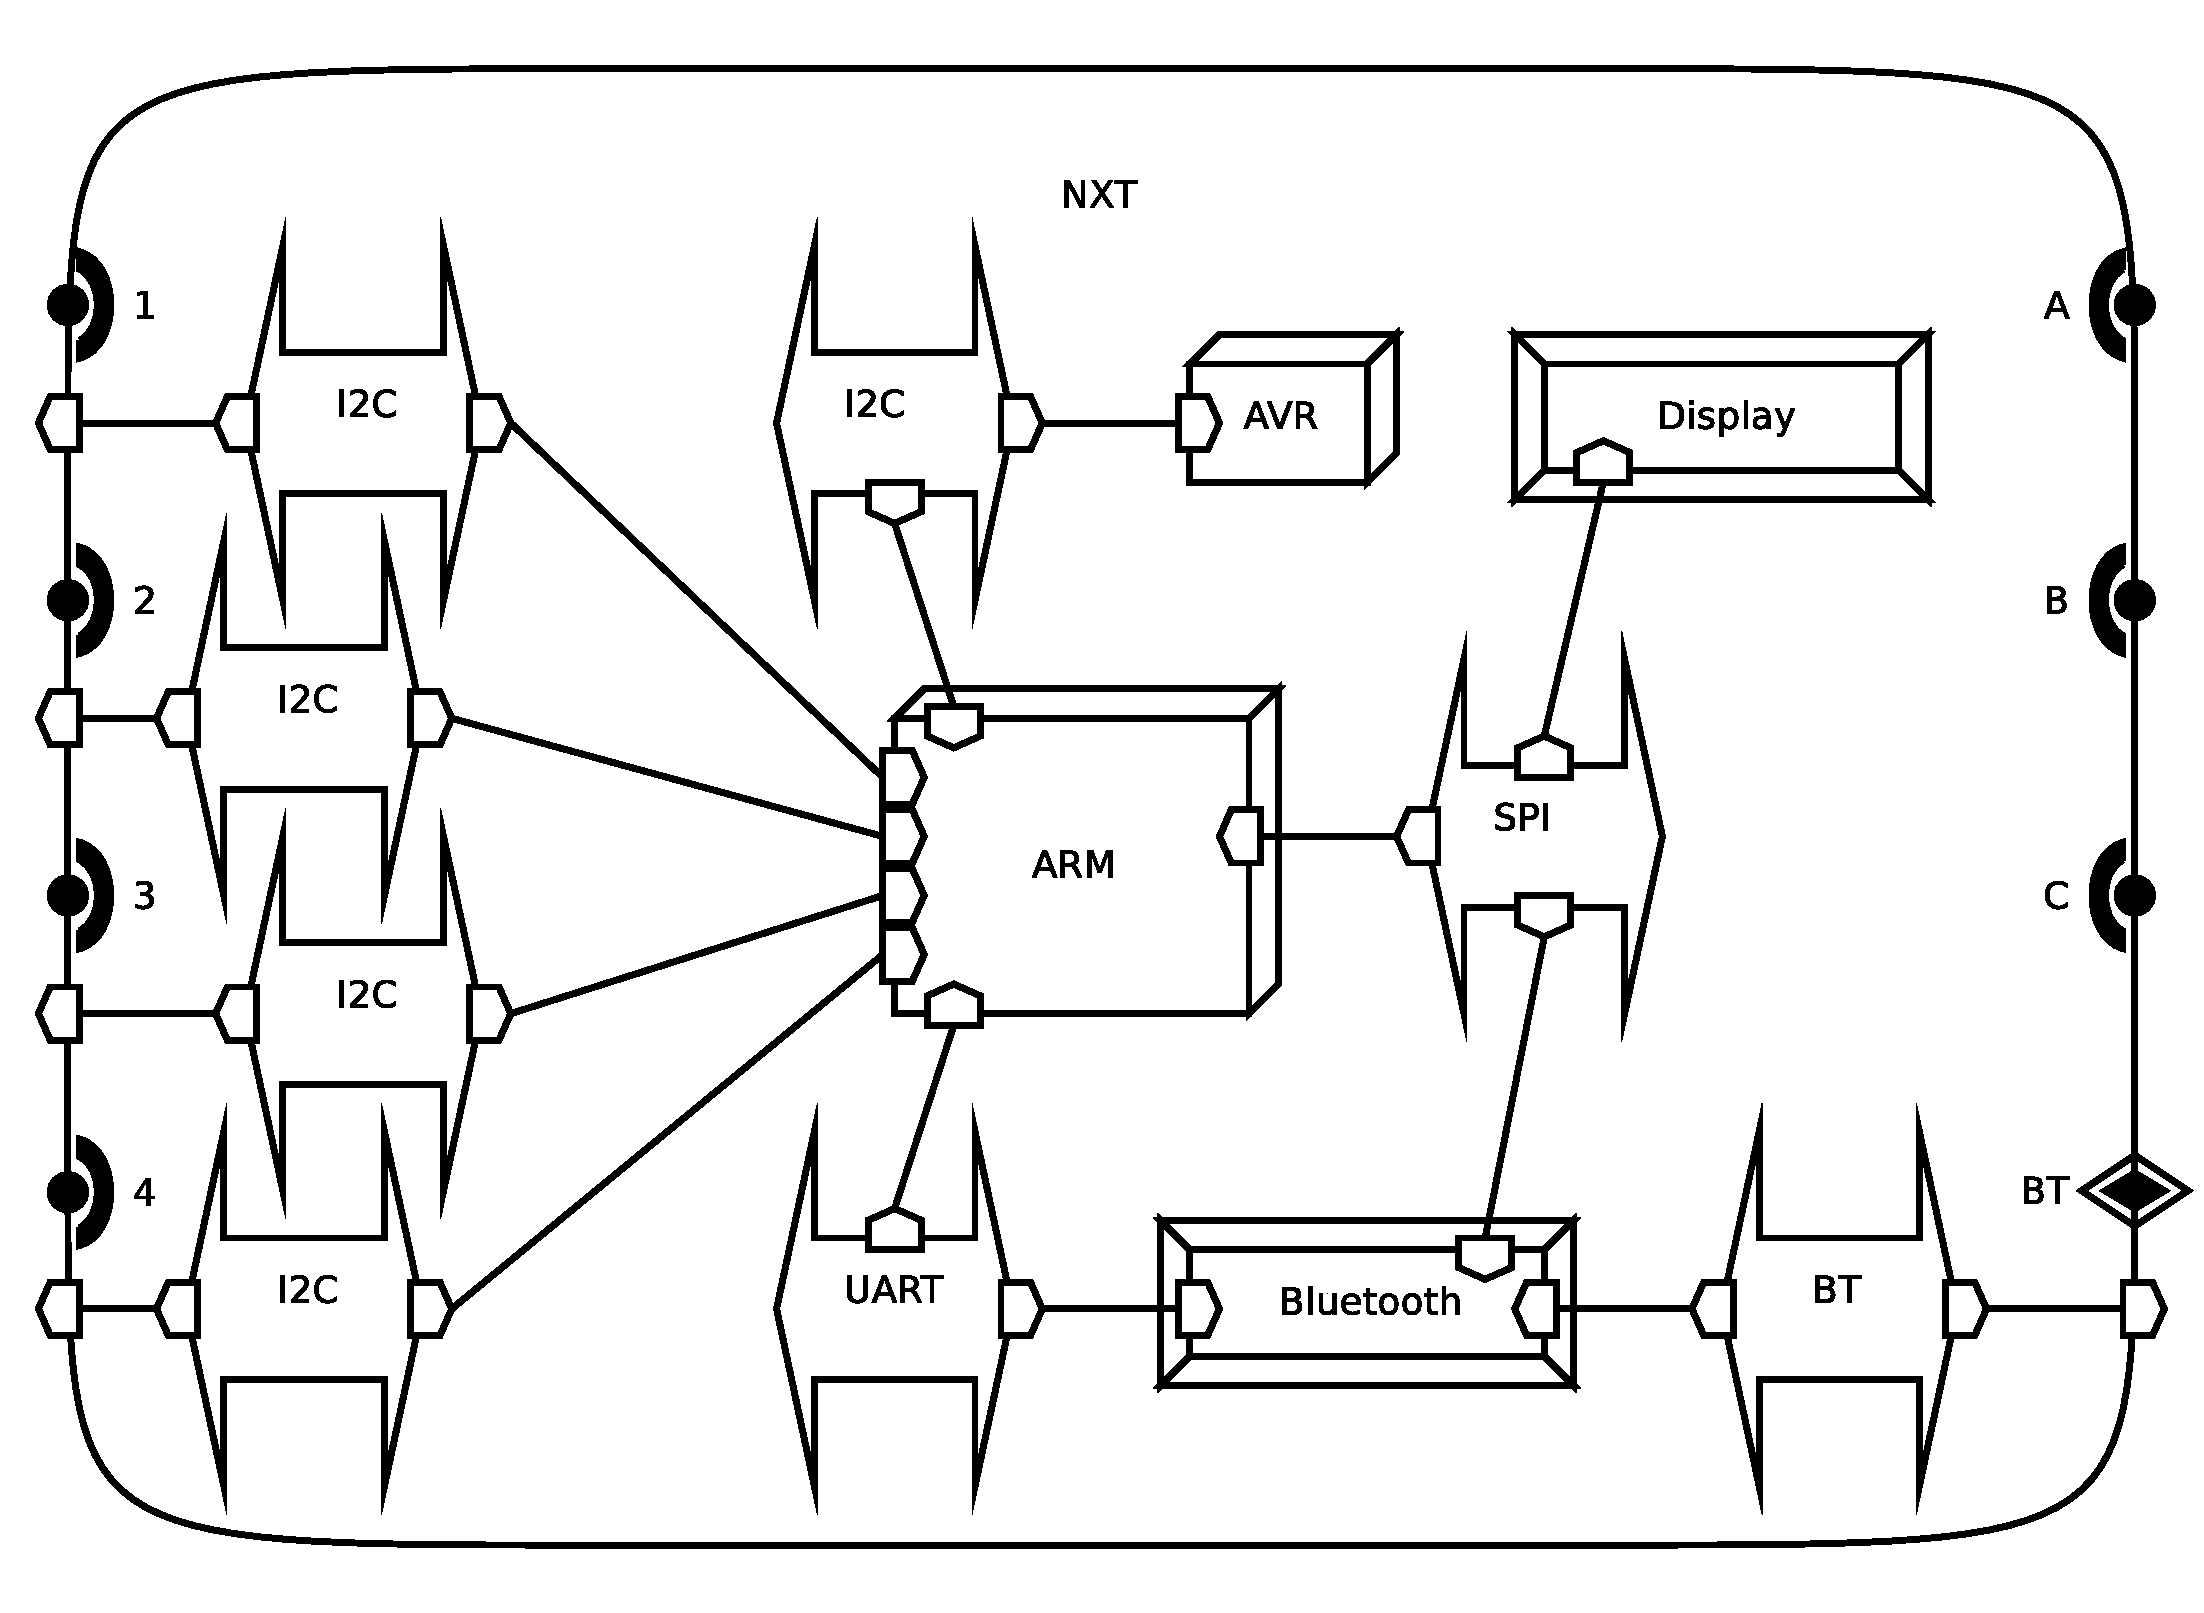
\includegraphics[scale=0.25]{./img/aadl-nxt1h.pdf}
        \caption{Modélisation AADL des composants matériels du NXT.}
        \label{fig:aadl-nxt1h}
      \end{figure}

      La figure \ref{fig:aadl-nxt1h} offre une représentation graphique du
      modèle matériel interne du {\it NXT}. Le composant principal est le
      processeur {\it ARM}, il est accompagné d'un coprocesseur ({\it AVR})
      ainsi que de différents bus et périphériques internes.

      L'ensemble des traitements est réalisés par le processeur. L'interaction
      avec certains périphériques est délégué au coprocesseur notamment avec les
      différents moteurs. Processeur et coprocesseur sont liés par un bus {\it
        I2C}. Le périphérique {\it bluetooth} interne est doublement lié au
      processeur par un bus {\it UART} et un bus {\it SPI}. Les groupes de
      ports d'entrées sont couplé chacun à un bus {\it I2C} qui les relient au
      processeur.

      ~

      \begin{figure}[!ht]
        \centering
        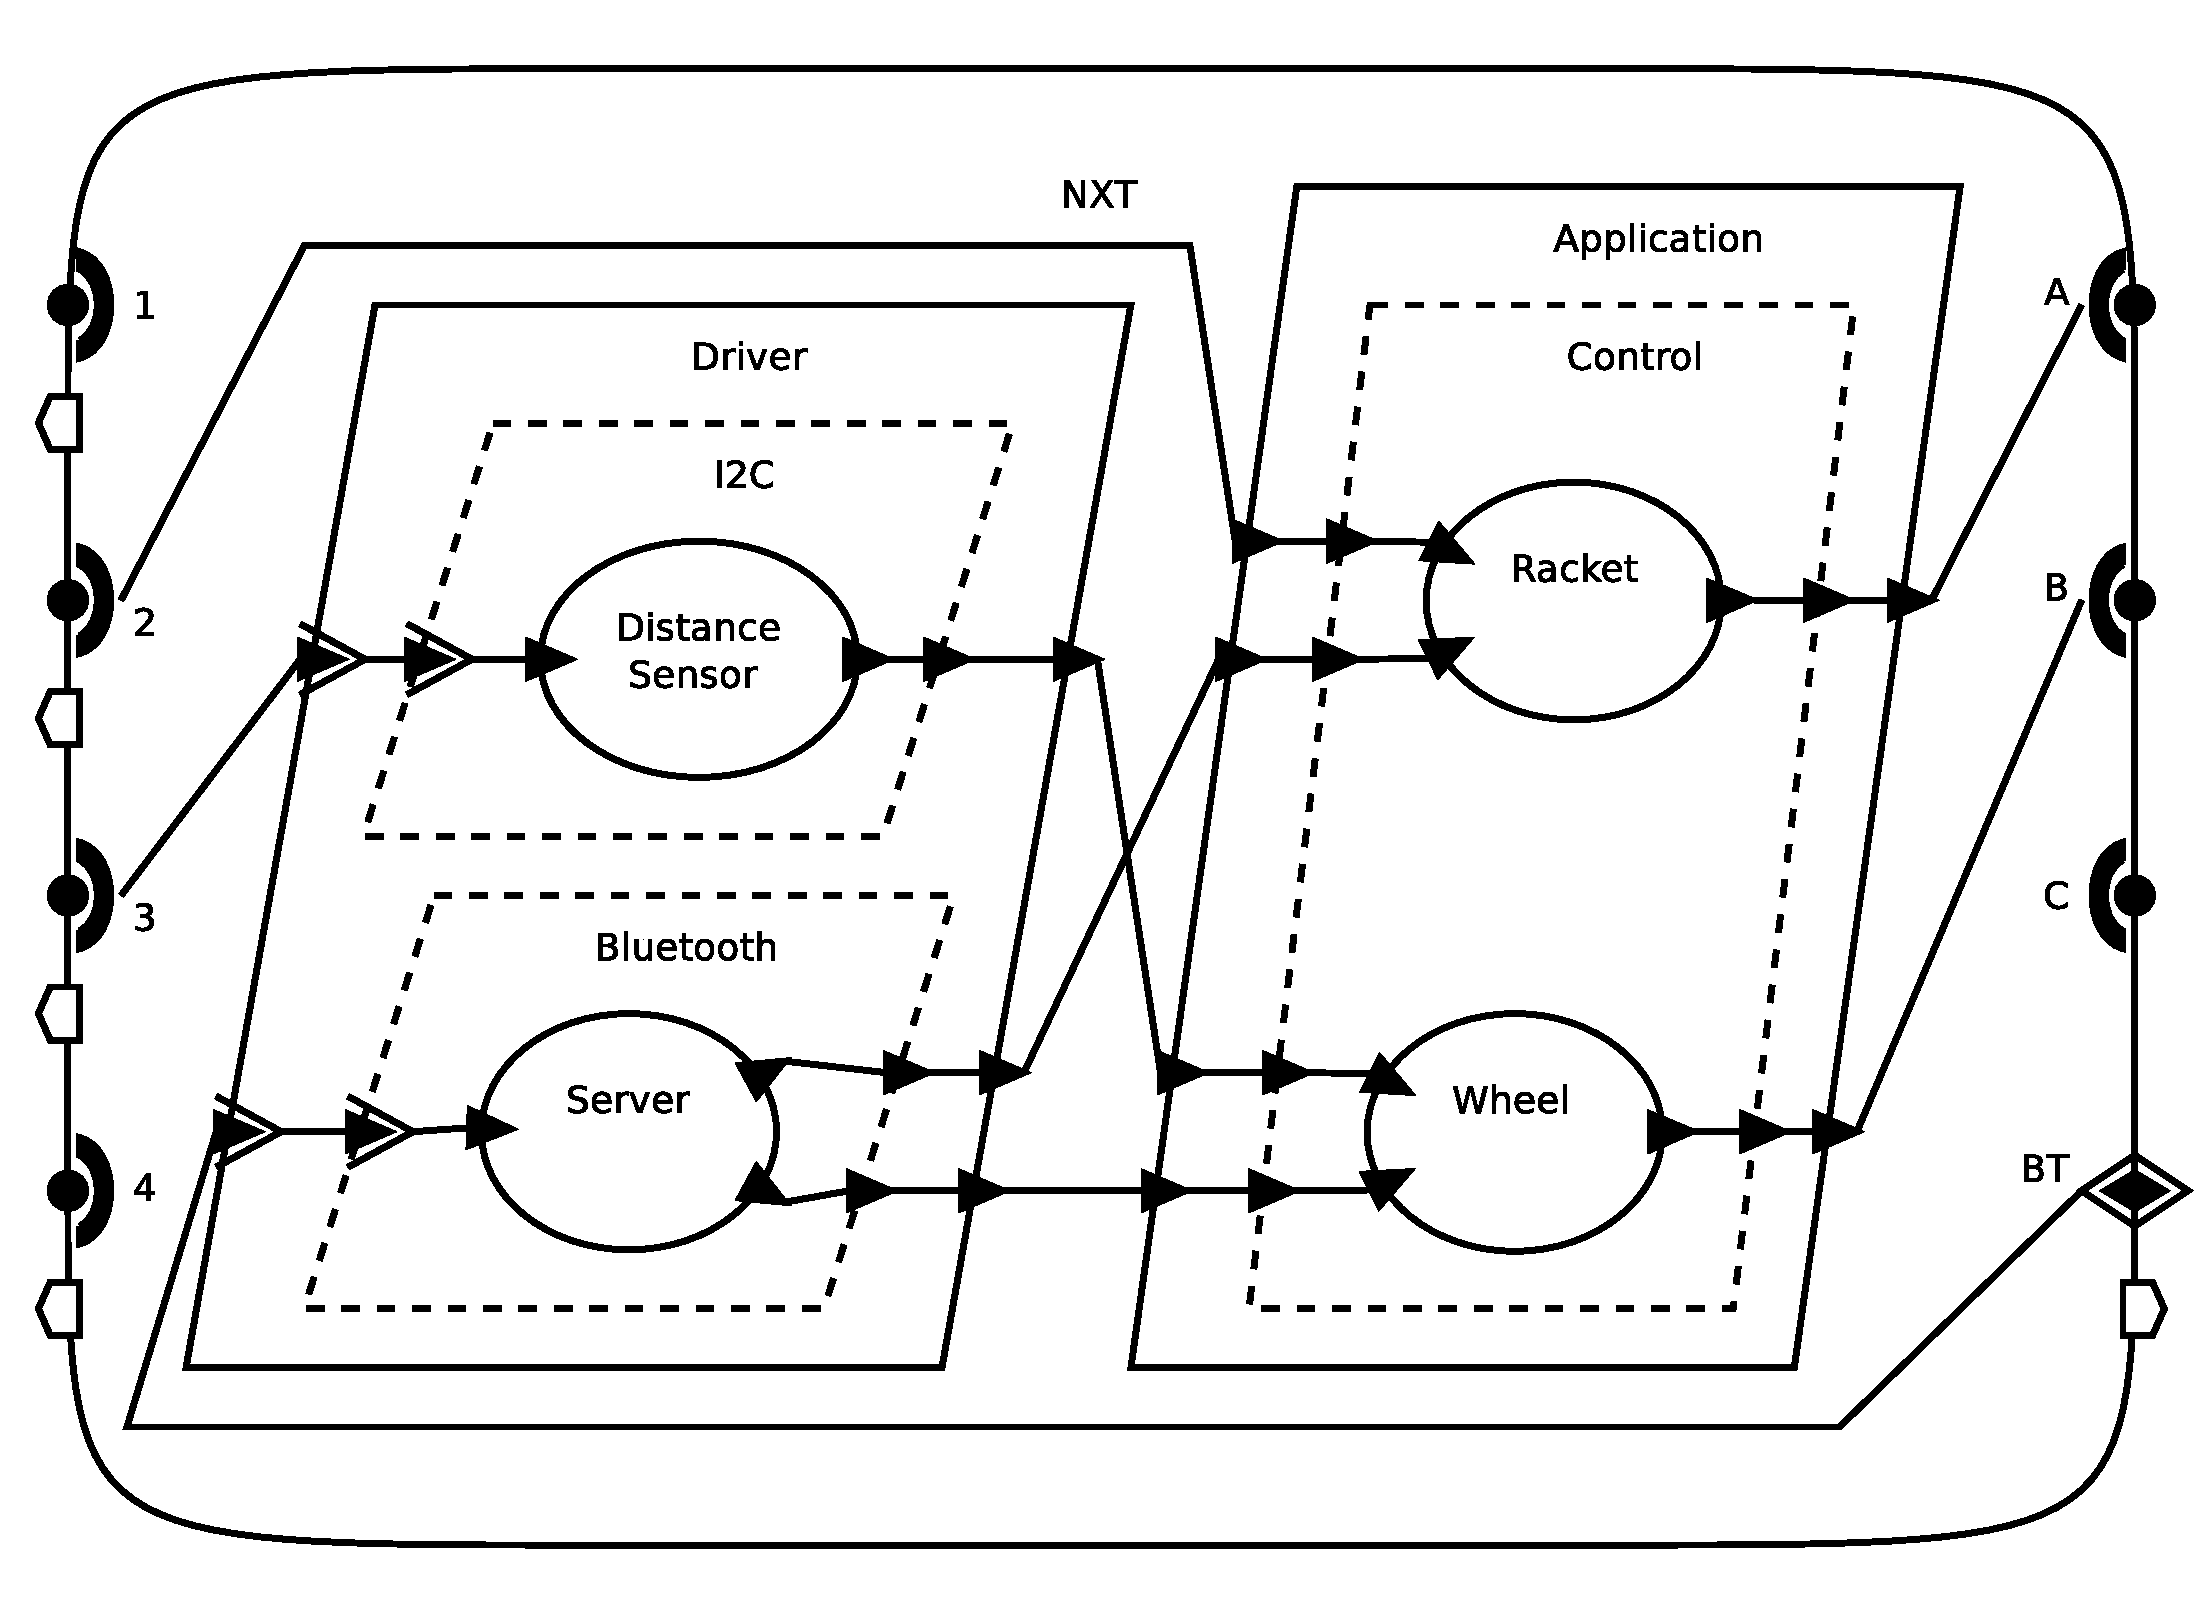
\includegraphics[scale=0.25]{./img/aadl-nxt1s.pdf}
        \caption{Modélisation AADL des composants logiciels du NXT.}
        \label{fig:aadl-nxt1s}
      \end{figure}

      La figure \ref{fig:aadl-nxt1s} offre une représentation graphique du
      modèle logiciel interne du {\it NXT}. Il est constitué de deux processus.
      Le premier processus ({\it Driver}) regroupe les pilotes de périphériques,
      il est composé d'une tâche pour le pilote {\it I2C} et d'une autre tâche
      pour le pilote {\it bluetooth}. Le seconde processus ({\it Application})
      contient la tâche d'asservissement du robot ({\it Control}).

      Le flux des données {\it bluetooth} lie le port d'entrée/sortie
      {\it BT} au processus regroupant les pilotes puis à la tâche du
      pilote {\it bluetooth}. Les données y sont traitées puis
      envoyées vers la tâche d'asservissement. Le flux des données
      {\it I2C} lie le groupe de ports {\it 3} au processus regroupant
      les pilotes puis à la tâche du pilote {\it I2C}. De la même
      façon, les données y sont traitées puis envoyées vers la tâche
      d'asservissement.

      La tâche d'asservissement contient deux sous-programmes. Le premier ({\it
        Racket}) récupère une donnée sur la proximité de la balle issue du pilote
      {\it bluetooth} et une donnée sur la position de la raquette issue du
      groupe de port {\it 2} et défini une vitesse à donner au moteur de la
      raquette sur le groupe de ports {\it A}. Le second ({\it Wheel}) récupère
      une donnée sur la position de la balle issue du pilote {\it bluetooth} et
      une donnée sur la position du robot issue du pilote {\it I2C} et défini
      une vitesse à donner au moteur de la roue sur le groupe de ports {\it B}.

      \subsubsection{Seconde spécification}

      \begin{figure}[!ht]
        \centering
        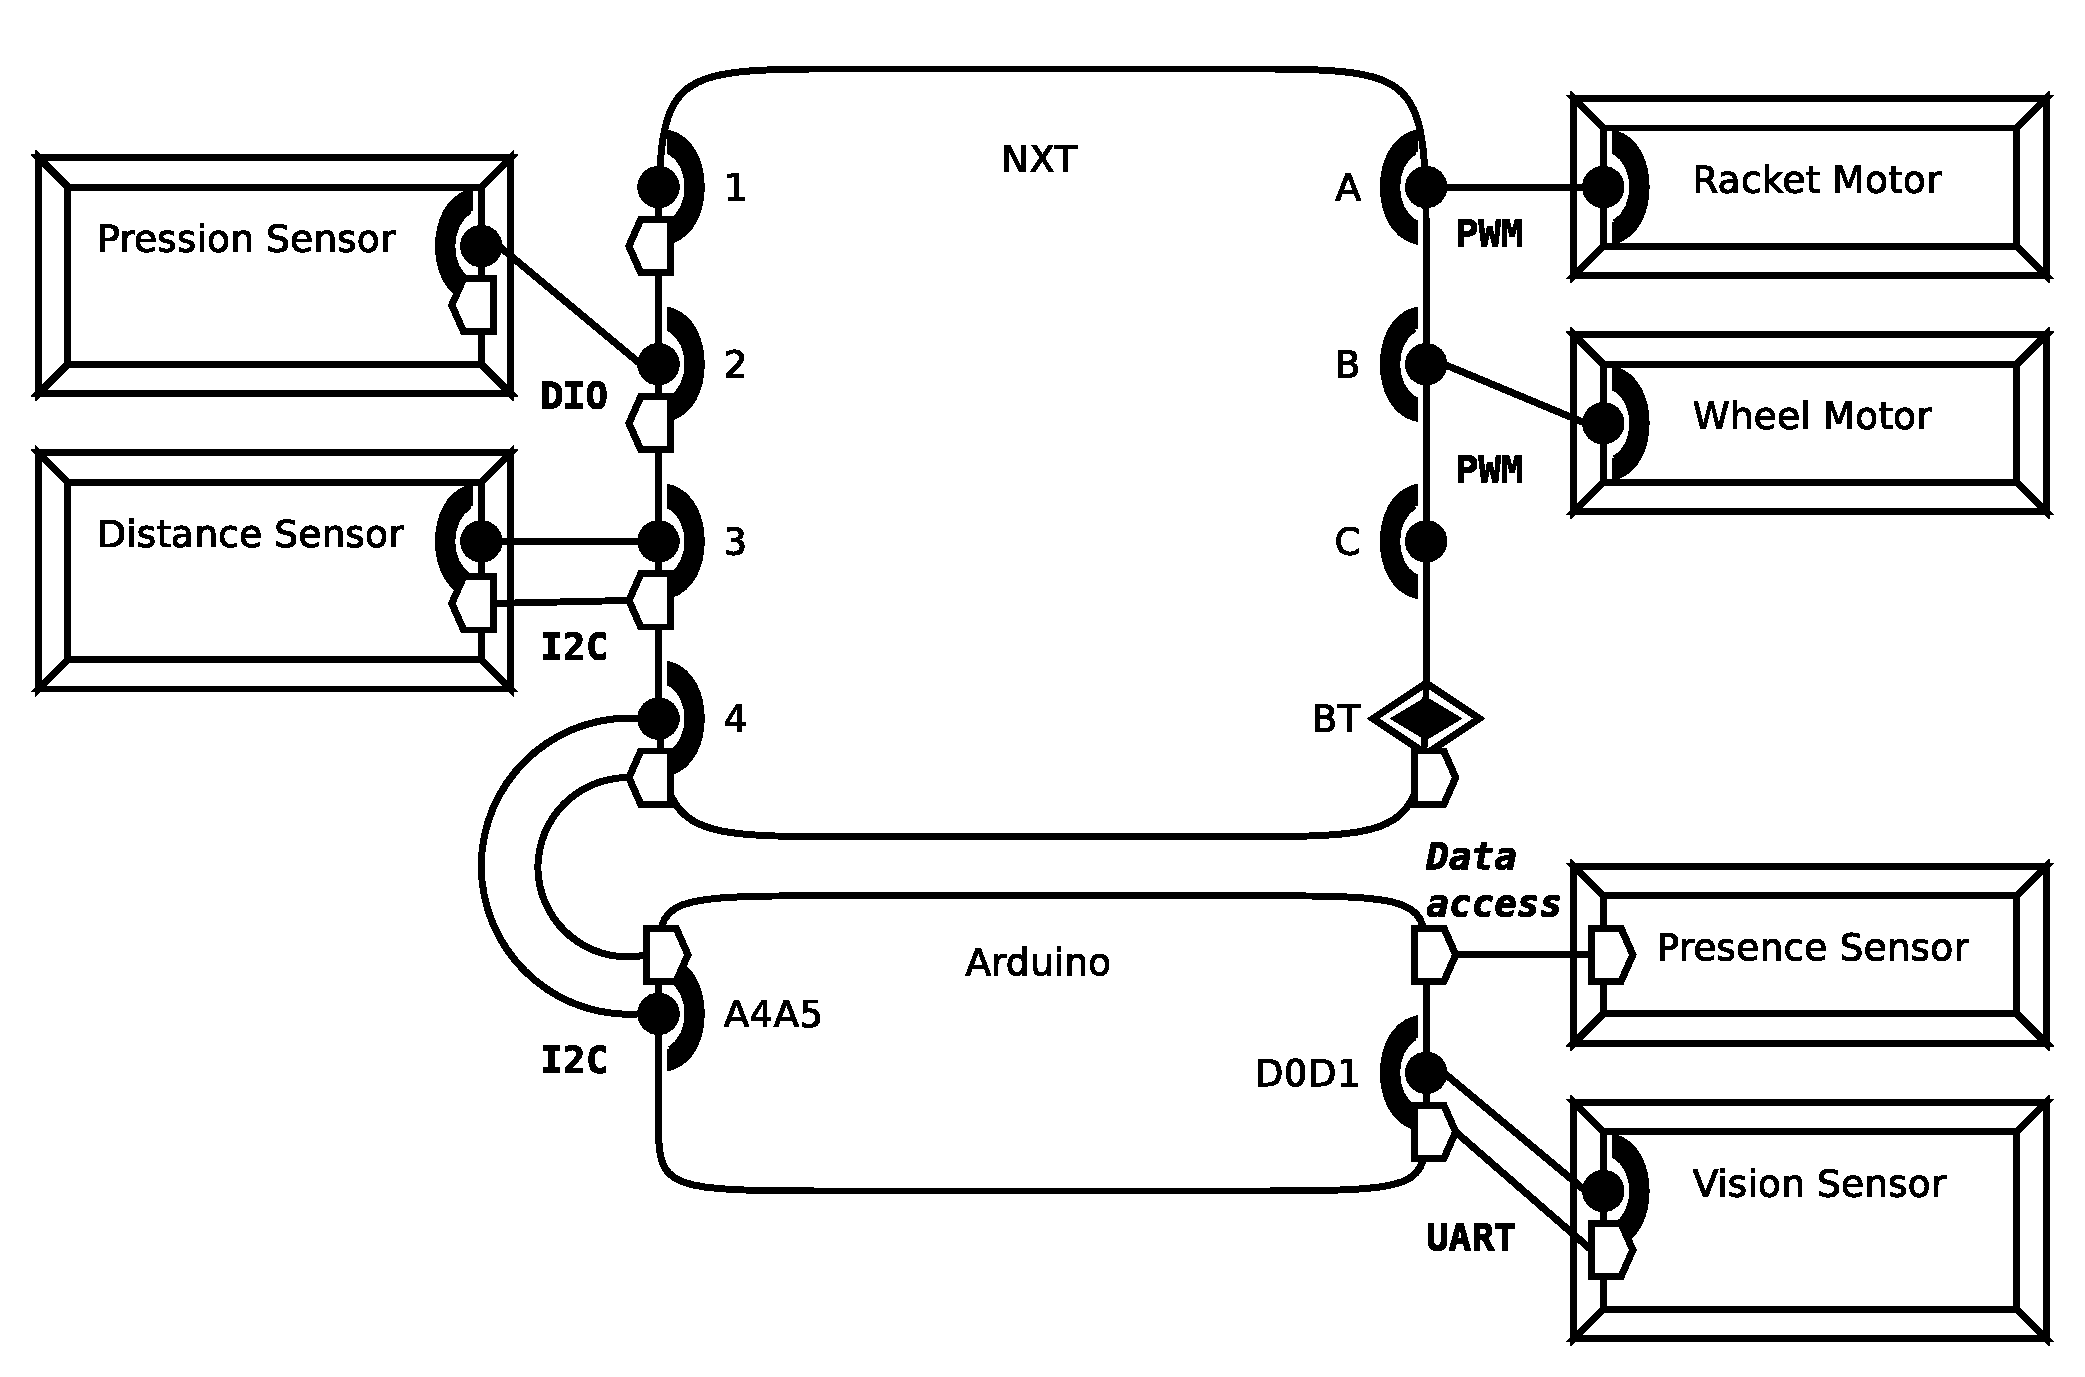
\includegraphics[scale=0.25]{./img/aadl-robot2.pdf}
        \caption{Vue global du système.}
        \label{fig:aadl-robot2}
      \end{figure}

      La figure \ref{fig:aadl-robot2} offre une représentation graphique du
      macro-modèle du robot suite à la modification de la spécification du
      démonstrateur. Celle-ci est semblable à la précédente à l'addition du
      système {\it Arduino} près. Le périphérique {\it bluetooth}, qui n'est
      plus utilisé, n'est plus représenté dans ce modèle.

      Afin de déterminer la position de la balle le système {\it
        Arduino} est couplé à deux périphérique. Une caméra ({\it Vision
        Sensor}) pour déterminer une position à distance du robot et une capteur
      de proximité ({\it Presence Sensor}) pour déterminer une position à
      proximité du robot. 

      Le flux de données et d'évènements entre la caméra et l'{\it Arduino} est
      réalisé par une connection sur un bus {\it UART}. Le capteur de proximité
      requiert un accès à une donnée interne à l'{\it Arduino}.  Le flux de
      données entre le système {\it Arduino} et le système {\it NXT} est réalisé
      par une connection sur le bus {\it I2C} du groupe de port {\it 4} dud
      système {\it NXT}.

      ~

      \begin{figure}[!ht]
        \centering
        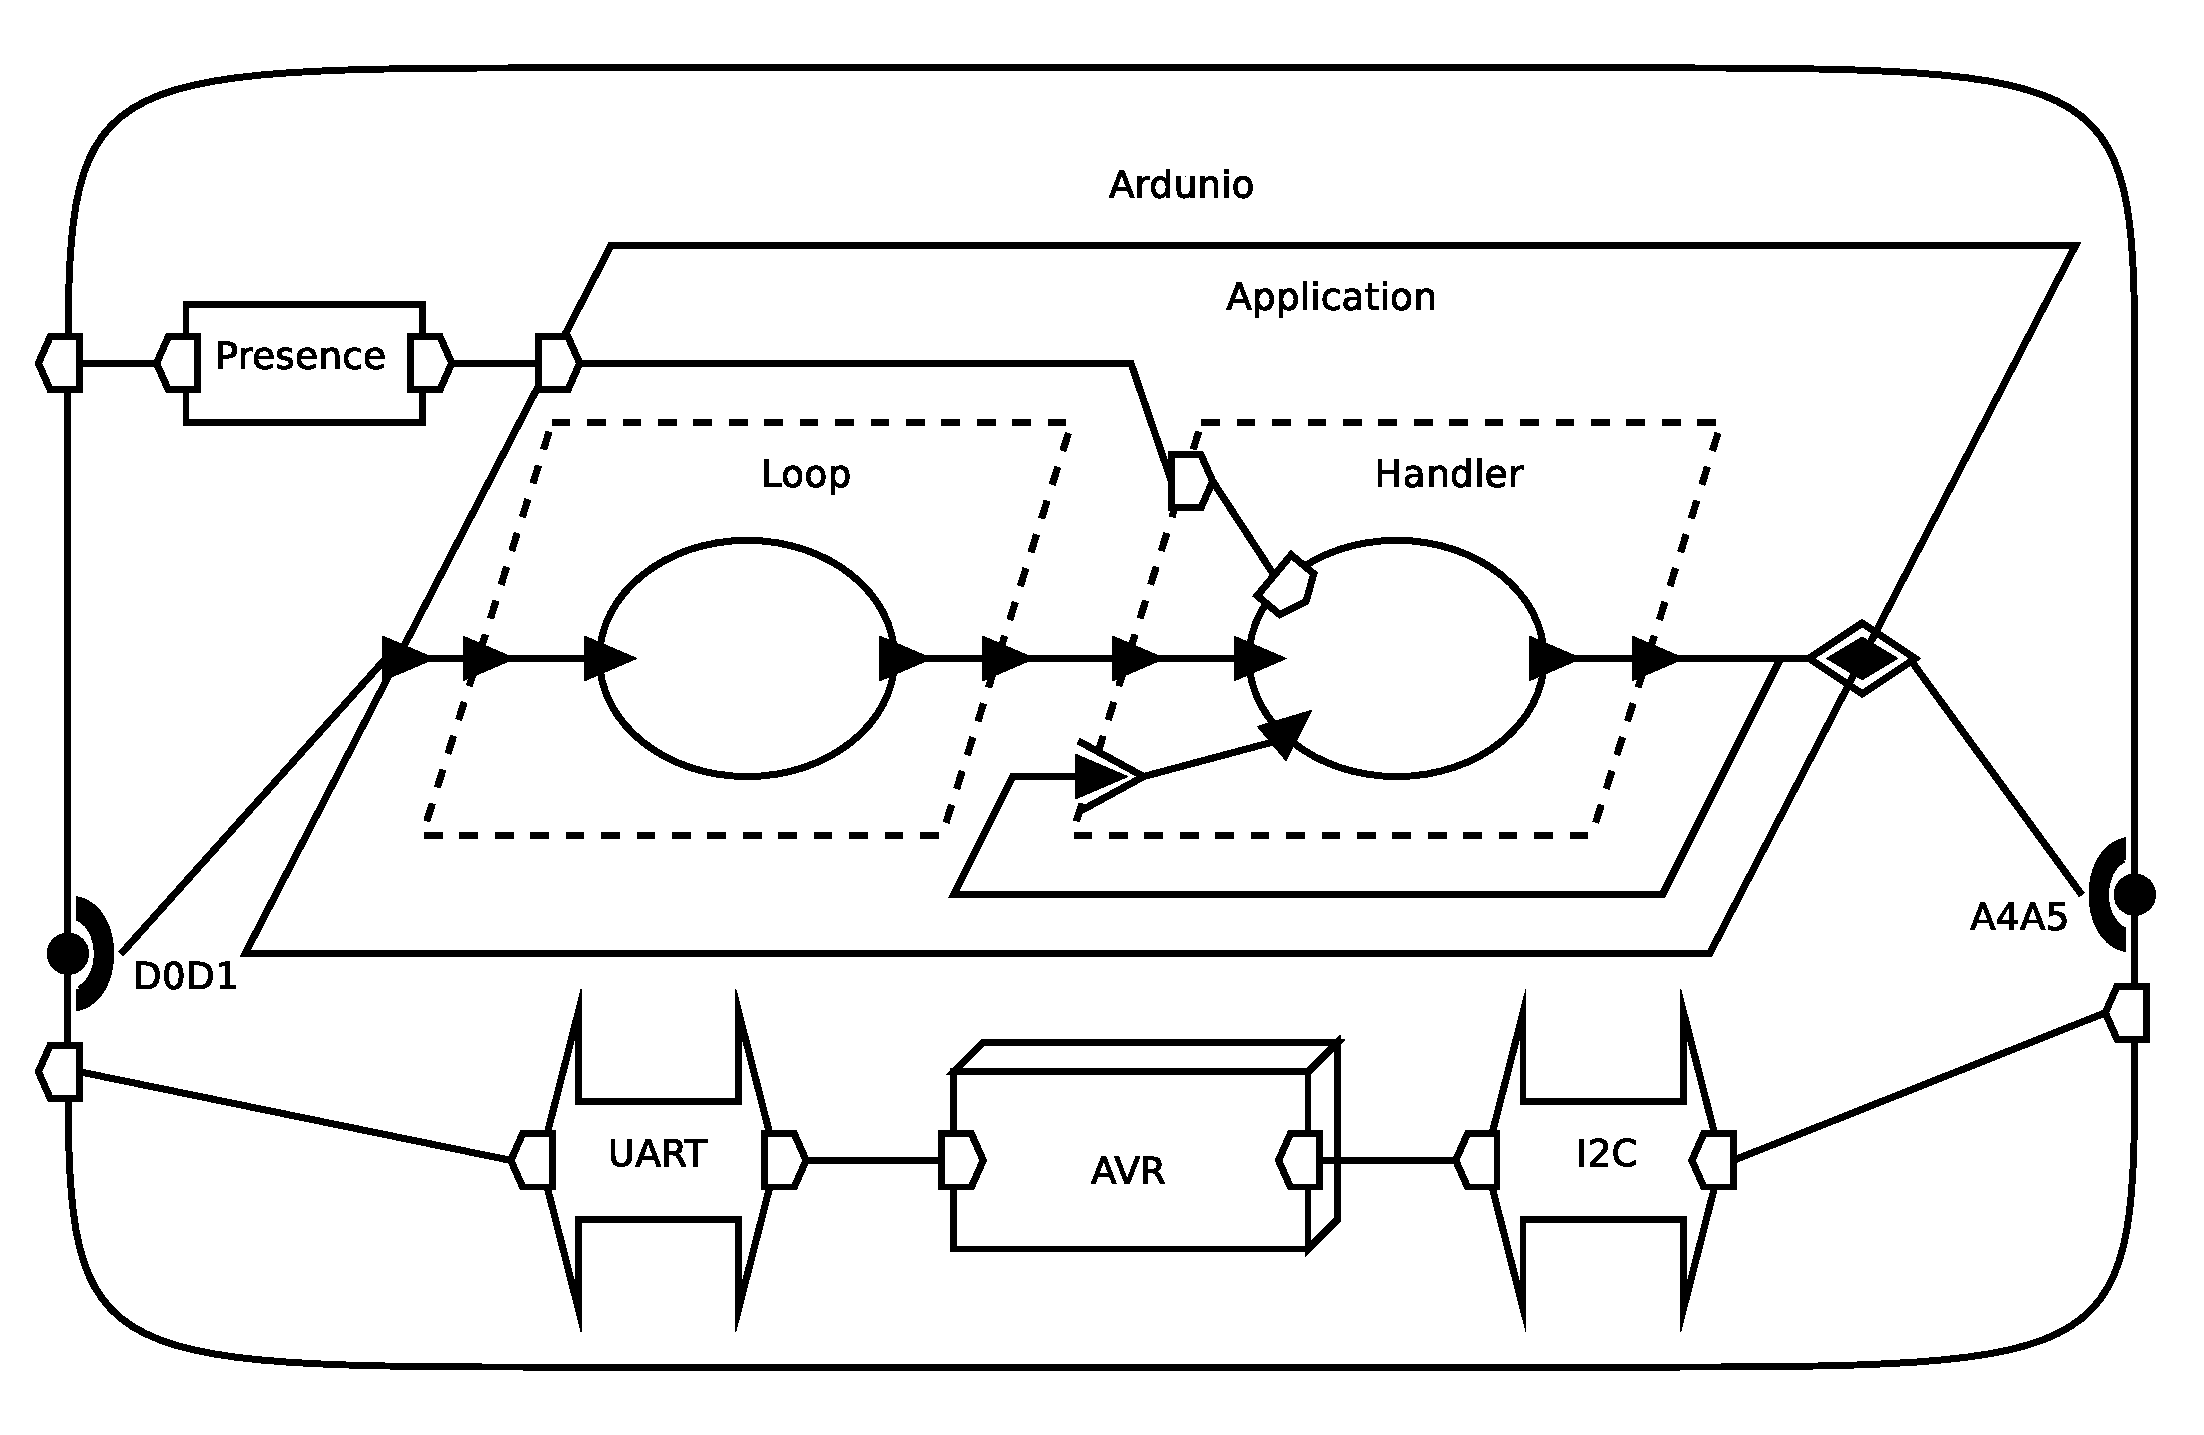
\includegraphics[scale=0.25]{./img/aadl-arduino.pdf}
        \caption{Modélisation AADL de l'Arduino.}
        \label{fig:aadl-arduino}
      \end{figure}
      
      La figure \ref{fig:aadl-arduino} offre une représentation graphique du
      modèle matériel et logiciel interne de l'{\it Arduino}. La composition
      matérielle de l'{\it Arduino} est relativement simple : il est constitué
      d'un microprocesseur {\it AVR} et de deux bus ({\it I2C} et {\it UART}).
      
      Il est constitué d'un processus ({\it Application}) reougroupant deux
      tâches. La première tâche ({\it Loop}) récupère les données issues de la
      caméra. La seonde tâche ({\it Handler}) est activée lorsqu'une requête est
      émise sur le bus {\it I2C}, elle retourne sur ce bus les données de la
      caméra et du capteur de proximité.
      
      ~

      \begin{figure}[!ht]
        \centering
        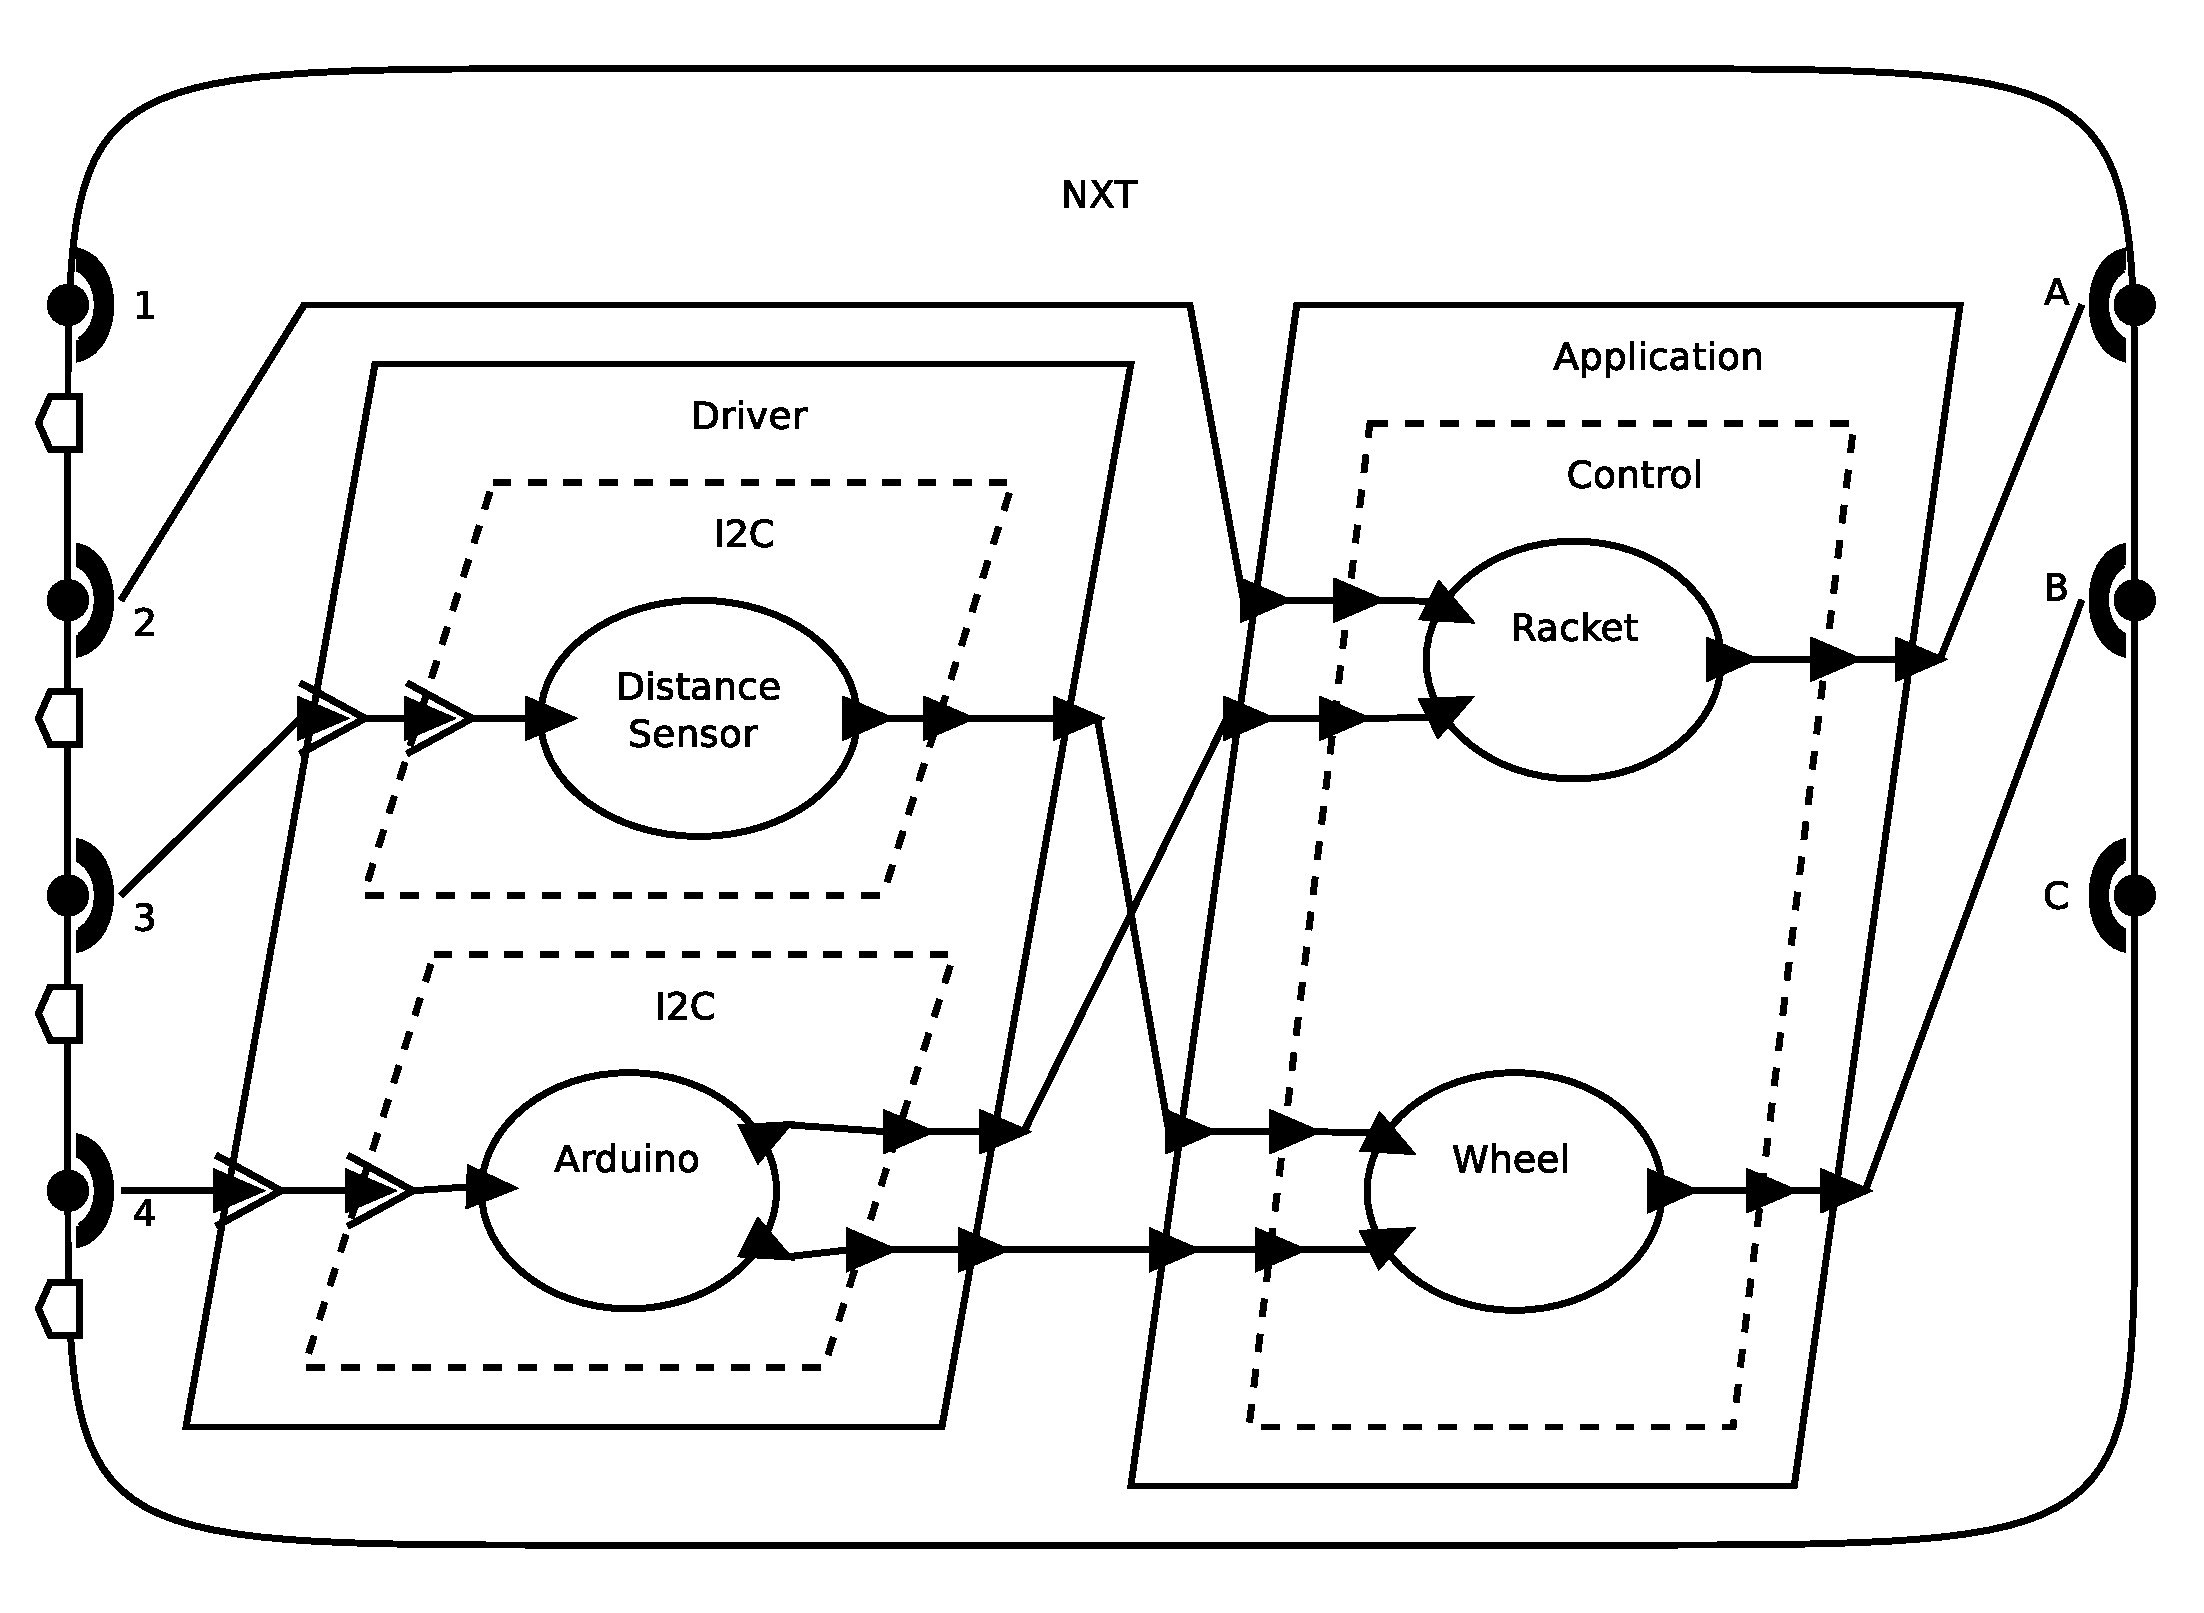
\includegraphics[scale=0.25]{./img/aadl-nxt2s.pdf}
        \caption{Modélisation AADL des composants logiciel du NXT.}
        \label{fig:aadl-nxt2s}
      \end{figure}

      La figure \ref{fig:aadl-nxt2s} offre une représentation graphique du
      modèle logiciel interne du {\it NXT}. De la même façon que dans le modèle
      correspondant de la première spécification il est constitué de deux
      processus. Le premier processus ({\it Driver}) regroupe les pilotes de
      périphériques, il est composé de deux tâches correspondant à deux
      instances du pilote {\it I2C}. Le seconde processus ({\it Application})
      contient la tâche d'asservissement du robot ({\it Control}).

      Le premier flux de données {\it I2C} lie le groupe de ports {\it 4} au
      processus regroupant les pilotes puis à l'instance du pilote {\it I2C}
      consacré à l'{\it Arduino}. Les données y sont traitées puis envoyées vers
      la tâche d'asservissement. Le second flux des données {\it I2C} lie le
      groupe de ports {\it 3} au processus regroupant les pilotes puis à
      l'instance du pilote {\it I2C} consacré au capteur de distance. De la même
      façon, les données y sont traitées puis envoyées vers la tâche
      d'asservissement.

      Le fonctionnement interne du second processus ({\it Application}) et
      sensiblement le même que dans le modèle correspondant de la première
      spécification. 
      
      ~

      Le travail de modélisation présenté ci-dessus présente partiellement le
      travail de modélisation réalisé. En effet, celui-ci a été produit dans le
      format textuel d'AADL. Il est en partie reproduit en annexe
      \ref{ann:aadl}, le travail complet étant accessible sous forme d'un projet
      Osate sur un dépot public\footnotemark. La modélisation produite a été
      validé par mes encadrants lors de différentes réunions de travail.
      \footnotetext{\url{http://github.com/LiberH/srsar/tree/master/models/aadl}}
      
      Il a été décidé de présenté ici certaines partie importante de ce travail
      de modélisation sous forme graphique de manière à être expliqué plus
      efficacement et compris plus facilement.
      
    \subsection{Modélisation comportementale}

      Afin de réaliser la modélisation comportementale c'est UPPAAL \cite{uppaal}
      qui a été choisi. UPPAAL, pour {\it Uppsala} et {\it Aalborg} les deux
      universités à l'origine de cet outil, est un environnement de modélisation
      pour le temps réel, les modèles manipulés sont réseaux automates temporisés.

      Le choix de cet outil résulte de plusieurs facteurs.  Le travail de
      modélisation attendu aurait pu être fait sous forme de réseaux de Petri et
      donc avec un autre outil, cependant, il m'a semblé plus naturel de le
      réaliser sous forme d'un réseaux d'automates temporisés. L'un des
      avantages de cet outil est son interface graphique qui intégre différents
      outils permetant de modéliser, simuler, et vérifier de manière simple et
      rapide le système considéré. Enfin, ayant déjà travaillé avec UPPAAL par
      le passé j'ai pu rapidement le reprendre en main.

      ~

      \begin{figure}[!ht]
        \centering
        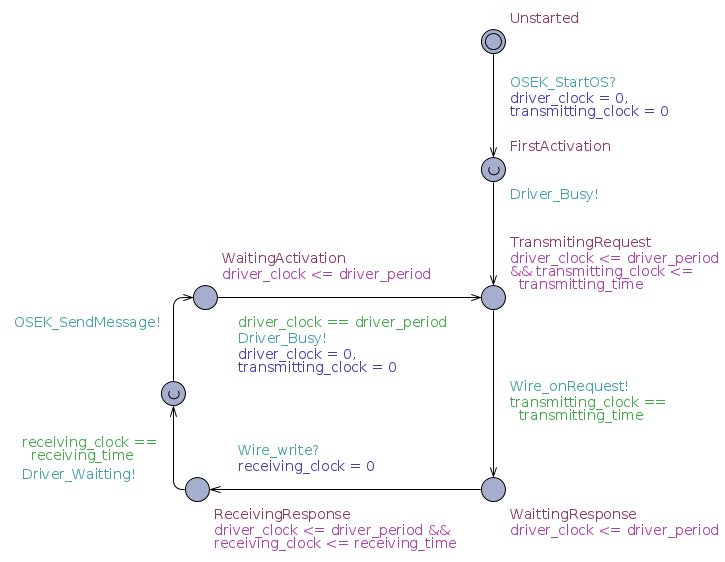
\includegraphics[scale=0.5]{./img/uppaal-driver.png}
        \caption{Modélisation de la tâche {\it I2C}}
        \label{uppaal-driver}
      \end{figure}
      
      
      La figure \ref{uppaal-driver} offre une représentation du modèle de la
      tâche {\it I2C} du NXT. Celle-ci joue le rôle de pilote de périphérique
      pour l'I2C.
      
      Initialement, l'état courant de
      l'automate est {\it Unstarted}. Un temps indéfini peut y être passé en
      attente du démarrage du système d'exploitation. Ce comportement est
      modélisé par la synchronisation de l'automate sur l'action
      {\it OSEK\_StartOS}. Lorsque le système d'exploitation démarre, l'action
      {\it OSEK\_StartOS} est réalisée, la transition est prise. L'automate
      se trouve alors dans l'état {\it FirstActivation}. Cet état est dit
      {\it urgent}, cela signifie que que la transition sortant de cet état
      sera prise dès qu'elle pourra l'être. Par construction, cette dernière l'est
      immédiatement, l'action {\it Driver\_Busy} est alors réalisée.
      Ce comportement modélise l'activation de la tâche {\it I2C} au démarrage
      du système d'exploitation.
      
      Cette tâche étant périodique, le modèle est contraint de ne jamais
      s'exécuter plus longtemps que sa période. Cela est modélisé par
      l'utilisation d'invariants ({\tt driver\_clock <= driver\_period}).
      
      ~
      
      Le nouvel état courant est {\it TransmitingRequest}. L'automate temporisé
      décrit une boucle modélisant quatres actions sucessives retournant en cet état. La
      première action, réalisée dans l'état {\it TransmitingRequest}, est la
      transmission de la requête I2C sur le bus associé. Ce comportement n'est
      modélisé que par un temps car le bus I2C est déterministe et son débit
      est connu. Il est donc possible de déterminer précisemment le temps que
      cette transmission prend. Une fois ce temps écoulé, l'action {\it Wire\_onRequest}
      est réalisée et l'état courant devient {\it WaitingResponse}.
      
      La seconde action, modélisée par un écoulement de temps dans ce nouvel état, est
      l'attente de la réponse du périphérique I2C. L'automate se synchronise
      alors sur l'action {\it Wire\_write} indiquant le début de la transmission de la réponse du
      périphérique. Une fois cette action réalisée, le nouvel état courant est
      {\it ReceveingResponse}.
      
      Cet état modélise la transmission de la réponse sur le bus I2C. De même
      que pour la transmission précédente, il est possible d'en connaitre exactement
      le temps d'exécution. Cette action n'est donc modélisée que par une attente. Une fois
      ce délai écoulé le pilote utilise une primitive du système d'exploitation
      pour envoyer un message à la tâche concernée ({\it Control}). Une fois ce
      message reçu par la tâche {\it Control}, l'état courant du pilote I2C est
      {\it WaitingActivation}.
      
      Dans cet état, c'est l'attente de l'échéance de la période qui est
      modélisée. Une fois cette attente terminée, le cycle reprend depuis l'état
      {\it TransmittingRequest}.
      
      ~

      \begin{figure}[!ht]
        \centering
        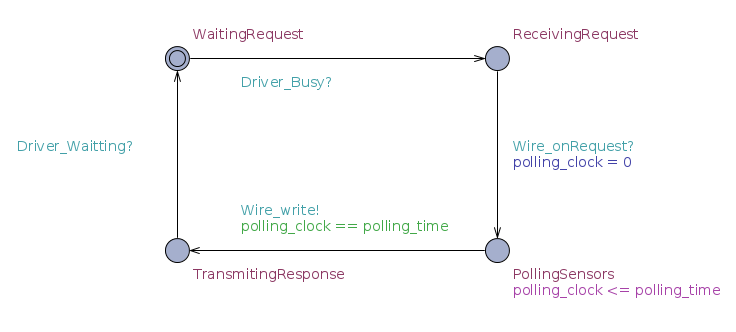
\includegraphics[scale=0.5]{./img/uppaal-handler.png}
        \caption{Modélisation de la tâche {\it Handler}}
        \label{uppaal-handler}
      \end{figure}


      La figure \ref{uppaal-handler} offre une représentation du modèle de la
      tâche {\it Handler} de l'Arduino. L'état initial de cet automate est
      {\it WaitingRequest}. Cette tâche est activée sur reception
      d'une interruption. Ce comportement est modélisé par une synchronisation
      sur action de mise en fonctionnement du pilote {\it I2C} du NXT
      ({\it Driver\_Busy}). L'état courant de l'automate est alors
      {\it ReceivingRequest}, un temps indéfini s'écoule dans cet état. C'est le
      temps de transmission de la requête évoquée dans la description du modèle
      du pilote I2C ci-dessus. Une fois ce temps écoulé, l'action
      {\it Wire\_onRequest} est réalisée par le pilote I2C, la transition est
      donc franchie dans cet automate et son état courant devient
      {\it PollingSensors}.
      
      Dans cet état l'Arduino interroge ses périphériques et construit la
      réponse à la requête I2C qu'il vient de recevoir. Une fois construite, il
      réalise l'action {\it Wire\_write} et débute la transmission de sa
      réponse vers le NXT. Son nouvel état courant est {\it TransmittingResponse}.
      
      À l'image du comportement observé dans l'état {\it ReceivingRequest}, il
      s'y écoule un temps défini dans le modèle du pilote I2C à la fin duquel
      le pilote réalise l'action {\it Driver\_Waiting}. Le nouvel état de
      l'automate est alors {\it WaitingRequest}. Le cycle reprend comme décrit
      ci-dessus.

      ~
      
      Le travail de modélisation décrit ici ne présente que partiellement le
      travail de modélisation réalisé. Les autres modèles réalisés sont reproduits en annexe
      \ref{ann:uppaal}. Le travail complet est accessible sous forme d'un projet
      UPPAAL sur un dépot public\footnotemark. La modélisation produite a été
      validée par mes encadrants lors de différentes réunions de travail.
      \footnotetext{\url{http://github.com/LiberH/srsar/tree/master/models/uppaal}}
      
      ~

      Lors de la production de ces modèles certaines problèmatiques ont été
      rencontrées. Par exemple, une question a été soulevée autour de la
      modélisation d'actions prennant un temps infime -- vis-à-vis des autres temps
      modélisés. Ne pas modéliser ces temps peut induire des comportements
      Zénon. Cependant, les modéliser implique soit de les modéliser plus grand
      qu'ils ne sont réellement, soit d'induire un écart important entre
      les plus petit et les plus grand temps modélisé. Cette dernière option a
      des conséquences significativement négatives sur l'efficacité des
      vérifications à réaliser sur le modèle considéré.
                  
      ~
      
      L'ensemble du comportement du démontrateur n'as pas été modélisé.
      En effet, les dynamiques de la balle et du moteur entrainant la roue ne sont pas
      modélisées. En l'état, s'il est possible de savoir si le robot frappe la
      balle lorsque celle-ci est à sa portée, il n'est cependant pas possible de
      savoir si le robot est effectivement placé en face de la balle lorsqu'il
      le fait.
      
      De telles dynamiques posent ici un problème de modélisation. En effet, elles
      ne peuvent pas être précisement modélisées par des modèles discrets. Or,
      les automates temporisés font parties de cette classe de modèles.
      Une solution peut être de discrétiser ces dynamiques. Cependant, cela
      implique une modélisation aproximée de la réalité et qui pourrait en être
      trop éloignée. Une autre solution évoquée au cours d'une réunion de travail
      est non-plus de modéliser la dynamique de la balle mais de réaliser un
      modèle statistique de la position de celle-ci.
      
  \section{Implémentation}
      
      Il était initiallement prévu que le démonstrateur soit fonctionnel avant
      le commencement de ce stage. Cependant, certains imprévus ayant fait
      contre-temps ont empêchés de produire le travail nécessaire sur le
      démonstrateur. Il était cependant nécessaire d'avoir un support sur lequel réaliser mes
      travaux. J'ai donc repris le travail de réalisation du démonstrateur,
      ce qui a partiellement modifié la nature de mon travail.
      
      ~
      
      La réalisation de cette implémentation a été chronophage et à
      ralenti mon travail vis-à-vis de ses objectifs initiaux. En effet,
      certains problèmes techniques, matériels comme logiciels, ont été
      rencontrés. Cela, que ce soit autour des objectifs du stage qui s'est
      déroulé en parallèle au mien, qu'autour d'autres problèmatiques de
      l'implémentation du démonstrateur. De fait une part importante de mon
      temps à été consacré à ce travail.
  
    \subsection{Implémentation matérielle}
 
      Le robot NXT Mindstorm de Lego a été développé pour initier les jeunes
      adolescents à la robotique et à la programmation informatique. Il a vite
      était repéré et récupéré par des adultes passionnés d'électronique ou de
      robotique pour son utilisation simple pouvant être facilement
      étendue. Afin de permettre une utilisation facile de son jouet, Lego a
      conçu le Mindstorm NXT comme suit : il y a une ``brique intelligente'', ou
      brique principale, concentrant l'ensemble des composants électroniques
      formant le ``cerveau'' du robot. Celle-ci peut-être reliée en USB à un
      ordinateur pour y déposer un programme. Elle comporte un écran et des
      boutons permettant de déterminer quel programme on souhaite lancer lors de
      l'utilisation du système d'origine ou pour piloter une application en
      cours d'execution.

      ~
      
      \begin{figure}
        \centering
        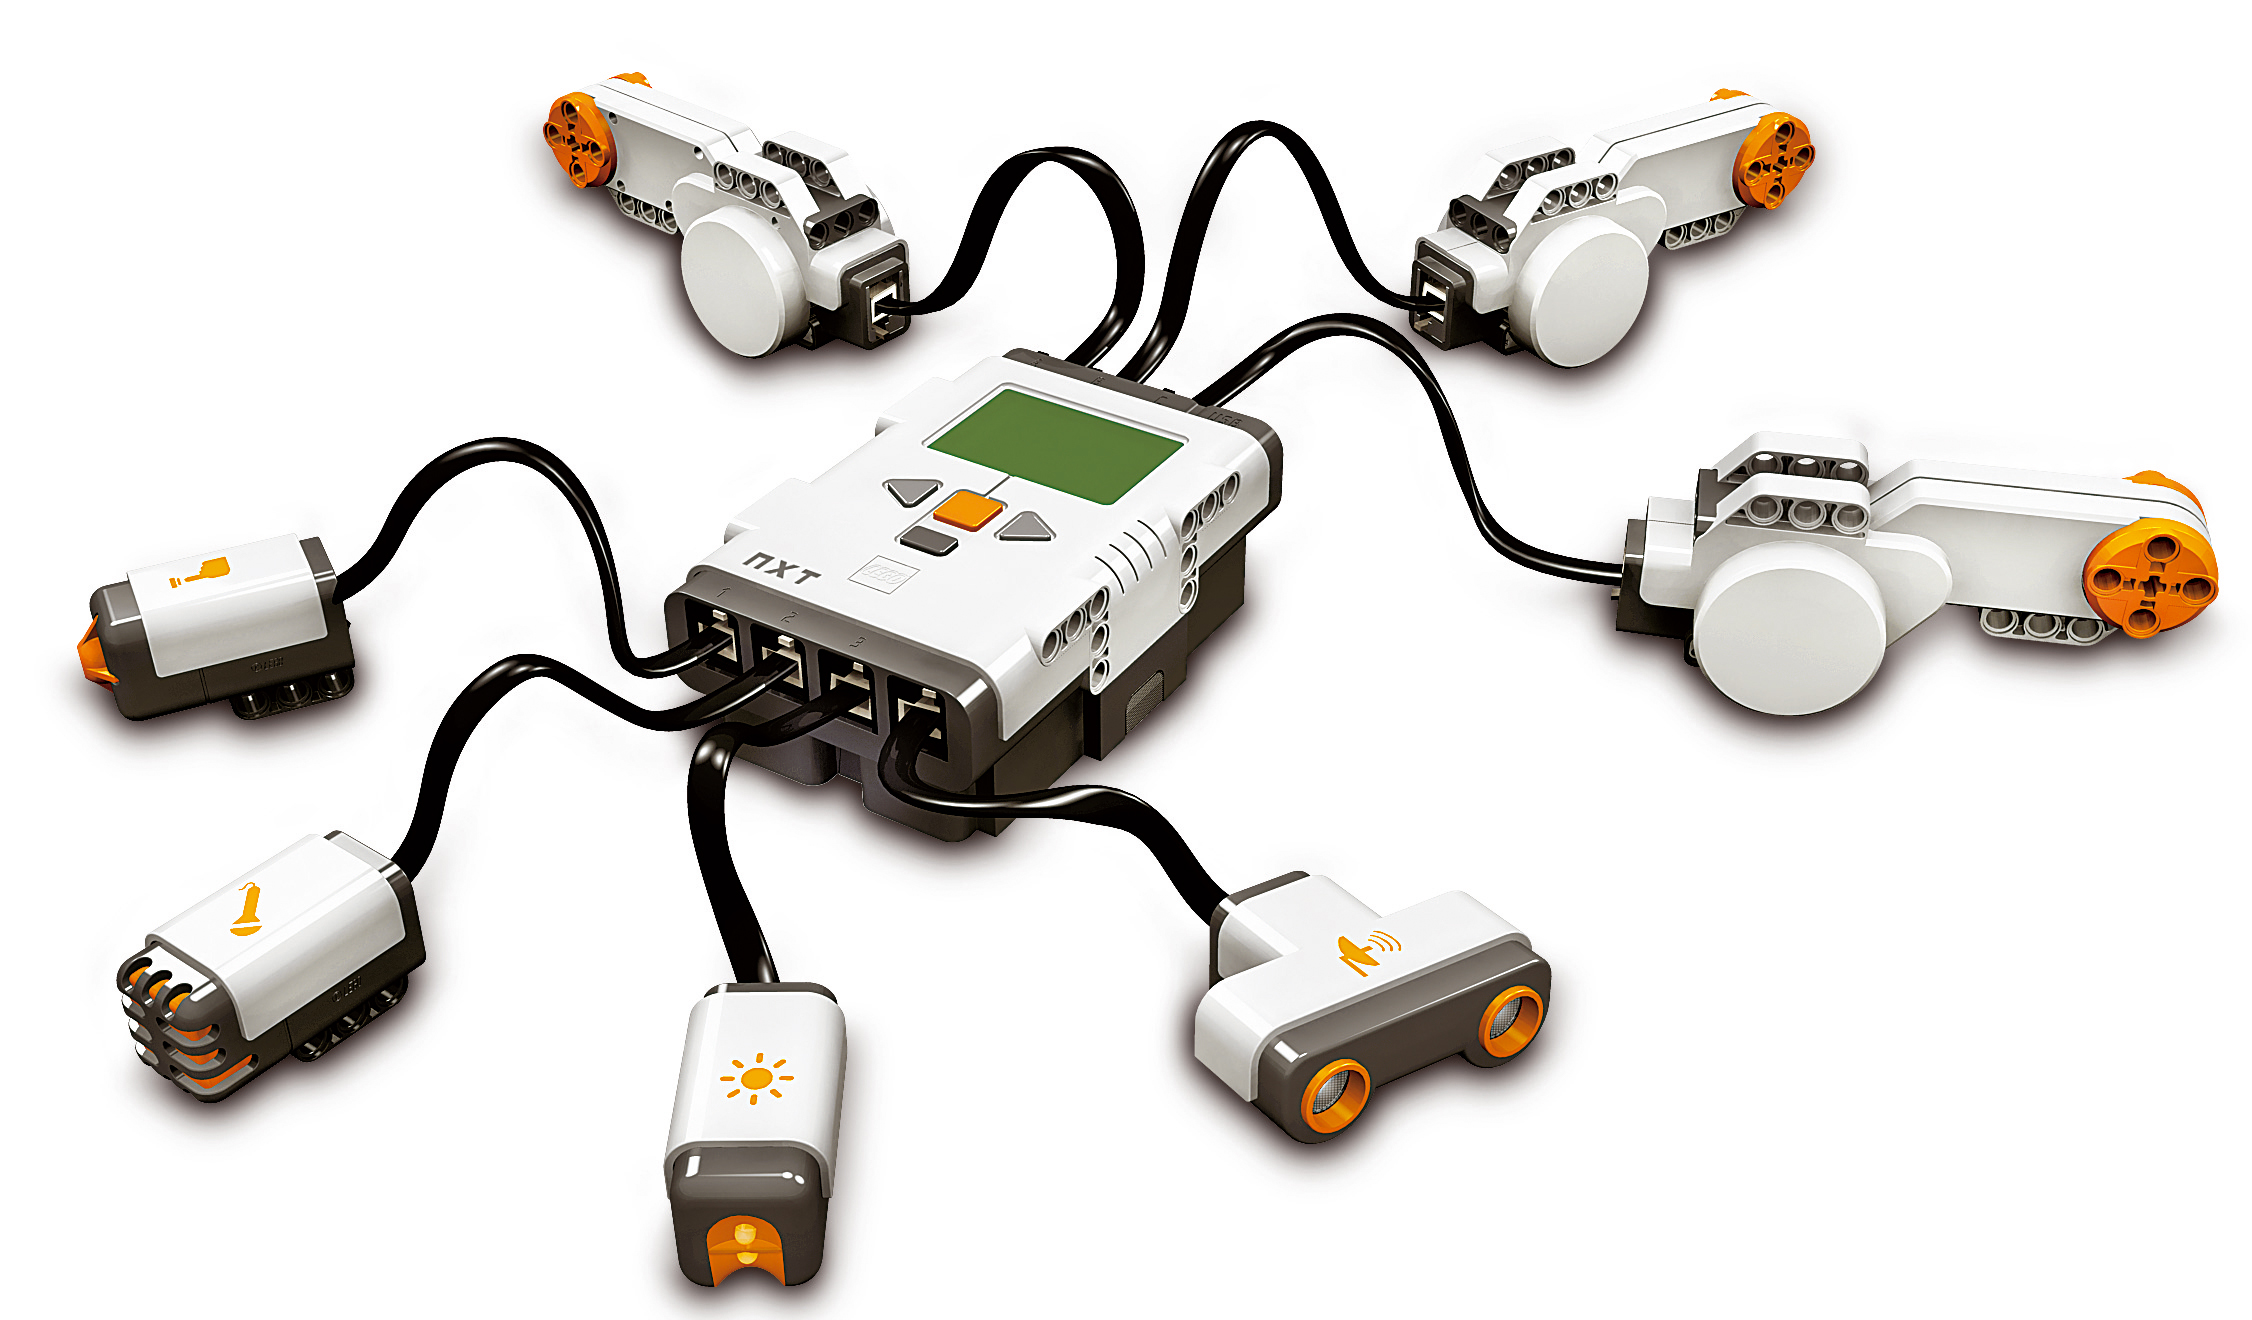
\includegraphics[scale=0.6]{./img/impl-nxt.jpg}
        \caption{Brique principale et périphériques du Minstorm NXT}
        \label{fig:impl-nxt}
      \end{figure}

      Sur cette brique peuvent être branchés des périphériques et plus
      précisemment 4 capteurs et 3 actionneurs. Leurs branchements sont
      facilités, utilisant tous les mêmes cables (RJ-12) comparables à des
      cables téléphoniques (RJ-11) -- voir figure \ref{fig:impl-nxt}. Mettant de
      côté les aspects complexes et fastidieux de la conception robotique,
      mécanique et électronique, il permet l'économie de leur mise en \oe uvre
      du point de vue du temps investi comme des moyens financiers
      engagés. C'est pour cet ensemble de raisons qu'il a été choisi le robot
      NXT en tant que composant intelligent du démonstrateur.

      ~
      
      \begin{figure}[!ht]
        \centering
        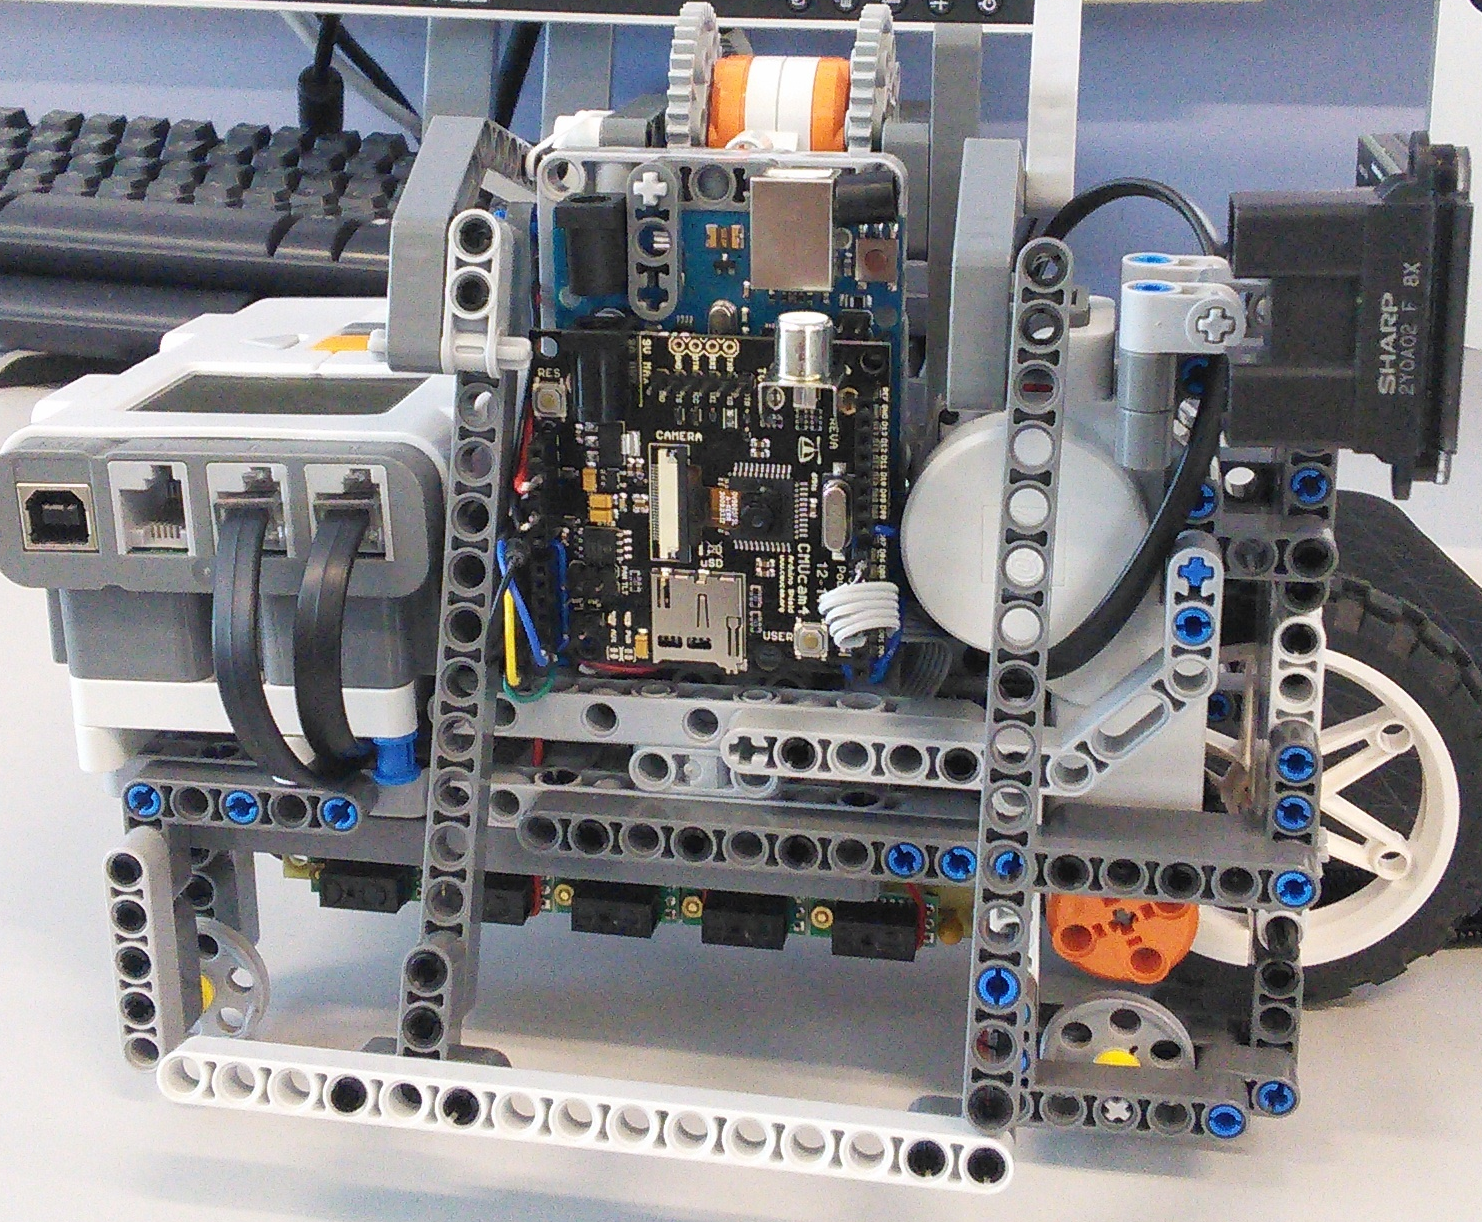
\includegraphics[width=0.8\textwidth]{./img/impl-robot.png}
        \caption{Une vue de l'implémentation matérielle du robot}
        \label{fig:impl-robot}
      \end{figure}
    
      Un second étudiant a travaillé sur l'implémentation matérielle du
      démonstrateur. Il a en effet participé à l'intégration de la caméra
      embarquée sur le robot NXT. Cette intégration a de fait modifié le
      démonstrateur -- voir figure \ref{fig:impl-robot}. Ces modifications ont
      été répércutées sur les différentes modélisations qui avaient été
      réalisées comme cela a pu être constaté ci-avant.

    \subsection{Implémentation logicielle}

      L'équipe Systèmes Temps Réel de l'IRCCyN travaille, entre autres choses,
      autour de ce qu'on appelle un système d'exploitation. C'est à dire une
      interface logicielle permettant d'abstraire l'utilisation des ressources
      matérielles -- électricité, espace mémoire, temps processeur, etc. -- d'un
      système physique. Le système d'exploitation que developpe l'équipe
      Systèmes Temps Réel a quelques particularités techniques le différenciant
      de celui que peut utiliser un ordinateur individuel standard.

      ~
    
      Ce système est conçu pour être utilisé sur des cartes électroniques ayant
      des usages plus restreints mais surtout plus spécifiques qu'un ordinateur
      personnel, étant lui capable de beaucoup de choses. Cette particularité en
      fait un système d'exploitation dit embarqué. L'informatique embarquée est
      présente dans les voitures, les trains, les avions mais aussi les
      téléphones intelligents très à la mode à notre époque. Au delà de ces
      exemples elle se cache dans beaucoup d'objets du quotidien. Cela en fait
      un enjeu majeur du point de vue économique mais aussi et peut-être avant
      tout pour le confort de vie de chacun à l'exemple de l'avion où l'embarqué
      est utile à assurer la sécurité de tous.

      ~
    
      Une autre spécificité de ce système est le fait qu'il soit temps réel. Le
      temps réel est une notion définissant un comportement particulier du
      système. Lorsque que l'on utilise un système temps réel on est assuré
      d'obtenir des résultats corrects dans des délais connus.

      ~
    
      Trampoline, le système developpé par l'équipe Temps Réel, fonctionne sur
      la plateforme Lego NXT ce qui permet une utilisation rapide et facile de
      ce dernier, que ce soit pour les chercheurs ou les étudiants.
      
  \section{Analyse}
    
    Afin de réaliser l'analyse de robustesse c'est Roméo \cite{gardey05}
    qui a été choisi. Roméo est un outil logiciel de vérification de modèles temporisés
    developpé au sein de l'équipe Système Temps Réel de l'IRCCyN. Il est utilisé pour
    vérifier des réseaux de Petri T-temporels. Il permet de mettre en \oe uvre
    des vérifications de modèles réalisant des synthèses de paramètres entiers
    bornés.

    C'est la vérsion 3.0$\alpha$ de Roméo qui a été utilisée. C'est une version
    en cours de développement. Certains problèmes ont été rencontrés lors
    de son utilisation retardant un peu l'obtention des premiers résultats.
    Cependant, ce travail a permis de tester cette nouvelle version de Roméo
    et d'en corriger certains petits défauts. Roméo étant une
    réalisation importante de l'équipe Système Temps Réel, le temps qui y est
    consacré n'est pour pas perdu.
    
    ~
    
    Une première étape nécessaire au travail d'analyse de la robustesse du
    modèle comportemental du démonstrateur est sa traduction vers un modèle
    équivalent manipulable par Roméo. Le modèle comportemental produit grace
    à UPPAAL est sous forme d'automates temporisés alors que Roméo manipule
    des modèles du type {\it Clock Transition System} \cite{lime12} (CTS) 
    adaptés à la vérification de réseaux de Petri T-temporels.
    
    La sémantique des automates temporisés définissent un écoulement du temps dans
    les localités qui le composent alors que dans les CTS définissent des intervales 
    de tirs sur les transitions qui les composent, à la manière des réseaux de
    Petri T-temporels.
    
    Le travail de traduction de modéle réalisé est reproduit en annexe
    \ref{ann:romeo}. Il est également disponible sur un dépot
    public\footnotemark. La modélisation produite a été
    validée par mes encadrants lors d'une réunion de travail.
    \footnotetext{\url{http://github.com/LiberH/srsar/tree/master/models/romeo}}
    
    ~
    
    Différentes propriétés ont été vérifiées sur ce modèle. Une première
    propriété a permis de s'assurer de l'absence d'interblocage dans celui-ci.
    Une seconde propriété à permis de monter une vivacité locale. Ainsi, on peut
    avancer que le service fourni par le pilote {\it I2C} (figure
    \ref{uppaal-driver}) est rendu infiniment souvent.
    
    Différentes synthèses de paramètres ont été réalisées avec ce modèle.
    Celles-ci ont été produite pour un paramètre et vérifiant la propriété
    d'absence d'interblocage. Les résultat obtenus nous indiquent, par exemple,
    que la période du pilote {\it I2C} fixé à 50 millisecondes peut être
    augementée ou diminuée de 10 millisecondes sans que la propriété d'absence
    d'interblocage ne soit invalidée.

    Ces résultats ne sont pas très significatifs quant à la la robustesse du
    modèle considéré. Ces synthèses constituent une analyse préliminaire de la
    robustesse du modèle du démonstrateur. Les résultats évoquées ont pu
    être obtenus sur un ordinateur de bureau. Cela autorise à penser que des
    synthèses de paramétres plus complexes pourront être réalisées 
    dans des temps acceptable quitte a utiliser pour cela une machine spécialisée.
         
    ~
    
    Des vérifications et synthèses de paramètres s'appuyant sur des propriétés
    quantitatives sont prévue à cours terme. L'ensemble des éléments nécessaires à leur
    réalisations sont aujroud'hui à disposition. Il est par exemple prévu de synthétisé un
    intervalle pour la période du pilote {\it I2C} vérifiant la propriété
    suivante : l'age des données collectées par l'Arduino sont traitées par le
    NXT avant une date fixée. Ce travail n'a pu être réalisé par manque de temps
    principalement dû aux divers problèmes liés à l'implémentation du
    démonstrateur.
    
    ~
    
    De la même façon, il n'a pas pu être produit d'analyse utilisant l'approche
    par réduction des automates temporisés implémenté dans l'outil Shrinktech \cite{sankur13}.
    Le travail à réaliser afin d'avoir à disposition tous les éléments nécessaires à cette
    analyse est plus important que dans le cas de l'utilisation de Roméo.
    En effet, il est nécessaire de prendre en main cet outil ainsi que sa syntaxe,
    de traduire le modèle comportemental vers celle-ci. Il est également
    nécessaire d'obtenir et de prendre en main l'outil Kronos \cite{yovine97}.
    En effet, l'outil Shrinktech est partiellement basé sur ce dernier.
    Shrinktech étant très récent et peu répendu, il peut ne pas avoir
    été testé extensivement. À la différence de l'utilisation de Roméo, ce
    travaille ne pourra être fait efficacement grace à une proximité direct
    avec l'auteur de l'outil.

  \section{Bilan}

    Ce document est organisé de manière à expliquer simplement le
    travail produit. Il évoque tout d'abord le travail de modélisation réalisé puis le
    travail d'implémentation produit et enfin le travail de vérification et d'analyse
    de robustesse entamé. Cependant, la production de ces travaux n'a pas été réalisée dans ce même
    ordre. Il a été nécesaire de réaliser l'implémentation matérielle et
    logicielle afin d'en modéliser l'architecture et le comportement.
    L'évolution de la spécification du démonstrateur et les contre-temps liés
    à son implémentation ont impactés sur le travail de modélisation et
    repoussé dans le temps le réalisation de l'analyse de robustesse du
    démonstrateur.
    
    ~
    
    La travail attendu quant à l'implémentation et la modélisation a été
    réalisé. Et il est envisageable à court terme de réaliser l'analyse de
    robustesse du démonstrateur.
    
    Dans le cadre de projets aux thématiques proches de celles étudiées par le
    projet ImpRo, il est prévu de poursuivre le développement du démonstrateur.
    Il est prévu de produire une implémentation matérielle à partir d'autres
    matériaux que les Lego Technics utilisés à ce jour. Lors d'utilisations
    prolongées des robots, les pièces Lego finissent par connaitre du jeu mécanique, voire
    parfois par se détacher les unes des autres.
    Il est également prévus de mettre au propre et compléter l'implémentation 
    logicielle afin qu'elle puisse être facilement réutilisée.
    
    Il est évoqué comme objectif à long terme de générer tout ou partie de
    l'implémentation logicielle des robots du démonstrateur afin d'assurer une
    distance minimale entre les modèles considérés et les implémentations qui
    en sont faites. 
    
    ~

    Lors de l'écriture du rapport bibliographique j'ai réalisé un travail de
    recherche. J'ai en effet produit une synthèse de littérature scientifique
    dans le domaine des modèles temporisés. Pour une part avec des travaux
    definissant les bases téoriques du domaine et pour autre part avec des
    travaus de l'état de l'art concernant la robustesse des modèles temporisés.

    ~

    Lors de la modélisation du démonstrateur j'ai réalisé un travail de
    conception et d'analyse. J'ai en effet produit un modèle architectural du
    démonstrateur grace au langage de conception d'architectures des systèmes
    embarqués et temps réel AADL. De même, j'ai produit un modèle comportemental du
    démonstrateur grace à l'outil de modélisation d'automates temporisés
    UPPAAL. J'ai traduit ce modèle sous une forme proche des réseaux de Petri
    afin d'en réaliser une analyse avec l'outil de vérification Roméo.

    ~

    Lors de l'implémentaion du démonstrateur j'ai également réalisé un travail
    technique. J'ai en effet participé à l'implémentation
    matérielle du démonstrateur mettant en \oe uvre des compétences en
    électronique et en moindre mesure en mécanique. De même, j'ai participé à
    l'implémentation logicielle du démonstrateur mettant en \oe uvre des
    compétences en programmation bas niveau, temps réel et en système.

    ~

    À travers la réalisation de ce stage j'ai pu mettre en \oe uvre différentes
    compétences acquisent au fils de mon cursus scolaire. Ce faisant, j'ai
    également pu consolider mais connaissances théoriques et mes compétences
    pratiques.

    Sur certains aspects de ce stage j'ai travaillé en autonomie. Cela m'a
    permis de mettre en place une organisation de mon travail personnel. Sur
    d'autres aspects j'ai pu collaboré avec un autre stagiaire ou avec mes
    encadrants.

    J'ai également été confronté à des contraintes techniques et des
    contre-temps. En accord avec mes encadrants, il m'a fallu faire des choix
    pour dépasser ceux-ci. Il m'a également fallu comprendre que cela peut être
    le déroulement normal de ce type de mission.


  
  \chapter*{Conclusion}
  \addcontentsline{toc}{chapter}{Conclusion}

    À travers ce stage j'ai pu acquérir de nouvelles connaissances et
    compétences dans le domaine des modèles temporisés. J'ai pu me confronter à
    la modélisation architecturale avec AADL et comportementale avec UPPAAL et
    Roméo d'une partie d'un système concret ainsi que réaliser des vérifications
    en utilisant des résultats de travaux de recherches de l'état de l'art.

    ~
    
    J'ai pu ainsi obtenir de solides bases théoriques dans ce domaine. J'ai
    également eu la chance de pouvoir assister à l'école d'été
    MOVEP\footnotemark qui se tenait à Nantes. Cette dernière a également
    participé à consolider mes acquis autour des méthodes formelles de
    modélisation et vérification des systèmes.
    \footnotetext{\url{http://movep14.irccyn.ec-nantes.fr}}

    ~
 
    Je suis très heureux d'avoir réalisé ce stage pour, et au sein de, l'équipe
    de recherche Systèmes Temps Réel de l'IRCCyN. Je suis également très
    heureux de poursuivre mon parcours dans cette même équipe dans le cadre d'un
    thèse.

  \appendix
  \chapter{Rapport bibliographique}
  \section*{Introduction}

    Ce rapport constitue un livrable dans le cadre d'un stage. Celui-ci
    s'integère au projet ANR ImpRo\footnotemark{} qui s'interesse aux problèmes
    liés aux implémentations des modèles formels de systèmes embarqués
    communicants.

    \footnotetext{http://anr-impro.irccyn.ec-nantes.fr}

    Ces modèles abstraient beaucoup d'aspects complexes ou de limitations de
    leur environnement d'execution. La modélisation du temps, en particulier,
    est habituellement idéale, avec des horloges infiniment précises, des tests
    ou des changements de mode instantanés. L'objectif de ce projet est
    d'étudier dans quelle mesure les implémentations de ces modèles préservent
    leurs propriétés.

    ~
    
    La robustesse d'un modèle caractérise l'importance de la différence existant
    entre ce modèle et la mise en \oe uvre qui en est faite. Cette difference
    réside, pour une part, dans l'écart entre la modèlisation d'un système et
    son implementation, pour une autre part, dans l'écart entre la modélisation
    de l'environement du système et l'environement réellement constaté. Si un
    écart faible ne permet pas de préserver les propriétés constater sur le
    modèle alors celui-ci est considéré comme peu robuste.

    ~
    
    Deux approches de robustesse des modèles temporisés développées dans le
    cadre de ce projet sont étudiés ici : la réduction des automates temporisés
    et la synthèse de paramètres temporels. Avant de les présenter, il est
    nécessaire d'introduire les concepts de base de la modélisation et la
    vérification des modèles temporisés.

    Pour ce faire, la section \ref{sec:modeles-temp} présente les concepts de
    base de la modélisation et de la vérification des modèles temporisés. La
    section \ref{sec:shrinking-timed-automata} présente une approche s'appuyant
    sur la réduction des bornes des contraintes temporelles. Enfin, la section
    \ref{sec:parameter-synthesis} présente la seconde approche qui se base sur
    la paramètrisation des contraintes temporelles.

  \section{Modèles temporisés}
  \label{sec:modeles-temp}

    \paragraph{Modélisation du temps.} ~
    
      ~

      Une approche pour modéliser le temps est de le discrétiser, on parle de
      temps discret. L'évolution du temps est représenté par une séquence
      d'entiers s'accroissant de manière monotone. Cette approche est appropriée
      pour certains types de circuits numériques synchrones où les changements
      des valeurs des signaux sont pris en compte à travers une observation
      synchrone.

      ~

      Évidemment, dans le cadres de processus physiques, les événements
      n'arrivent pas toujours à des dates d'horloges prenant leurs valeurs dans
      l'ensemble des entiers. La discrétisation du temps permet d'approximer le
      temps continu en choisisant a priori un quantum fixe ce qui limite la
      précision avec laquelle un système physique peut être modélisé. De fait,
      les interactions nécessitant une résolution plus fine du temps sont
      approximées.

      ~

      Une autre approche pour modéliser le temps est le temps dense. C'est un
      modèle plus naturel pour modéliser les processus physique opérant en temps
      continu. Les dates d'occurences d'évenements sont prises dans l'ensemble
      des nombres réels. De la même façon ils s'accroissent de manière
      monotone sans limite maximale. Ici, c'est cette dernière approche qui est
      considérée.

    \paragraph{Vérification des modèles temporisés.} ~

      ~

      La vérification de modèles est une approche fréquemment utilisée pour la
      vérification de propriétés d'accessibilité. Étant donné un système, la
      vérification d'une propriété d'accessibilité est réalisée par une
      exploration exhaustive de l'espace d'états du système.

      ~

      L'espace d'état d'un système correspond à l'ensemble des états possibles
      dans lesquels le système peut se trouver. Pour les automates temporisés,
      ces espaces d'états sont infinis. Ceci est dû à l'infinité de valeurs que
      peut possiblement prendre une horloge. Il est evidemment impossible de
      réaliser une enumération exhaustive des états d'un espace d'état infini.

      ~

      Pour faire face à ces problèmes différentes abstractions de l'espace
      d'état ont été proposées. Une vérification de modèle utilisant ces
      abstractions consiste alors à l'exploration d'un d'espace d'états abstrait
      équivalent significativement plus restreint. Ces abstrations consistent à
      regrouper des valuations d'horloges par classes d'équivalences. Il est
      donc nécessaire de trouver des classes d'équivalences à la fois efficaces
      et expressives.

      ~

      Quand bien même des méthodes abstraitisant cet espace infini sont
      utilisées, la taille de l'espace d'état abstrait équivalent croit
      exponentiellement avec de nombreux paramètres liés au système considéré
      comme leur nombre d'horloges et la taille des constantes auxquelles ses
      horloges sont comparées. Il est alors souvent trop couteux en temps et en
      mémoire de réaliser une vérification de modèle. Ce problème est appelé
      explosion de l'espace d'états.

    \paragraph{Notations formelles.} ~

      ~

      Une execution d'un système temporisé peut être définie en
      tant qu'un mot temporisé. Un mot temporisé sur un alphabet $\Sigma$ est
      une séquence $\omega = (\sigma_0,t_0)(\sigma_1,t_1)\dots(\sigma_n,t_n)$
      telle que $\forall i, \sigma_i \in \Sigma, t_i \in \mathbb{R}_{\geq 0}$ et
      $t_{i+1} \geq t_i$.

      ~

      Les mots temporisés sont reconnus par les systèmes de transitions
      temporisés. Ceux-ci sont les modèles élémentaires de description des
      systèmes temporisés, en effet, les autres modèles expriment leur
      sémantique sous forme de systèmes de transistions temporisés.
      Un système de transitions temporisés est un tuple $\tau = (S, s_0, \Sigma,
      \rightarrow)$ tel que :

      \begin{itemize}
        \item $S$ est un ensemble fini d'états ;
        \item $s_0\in S$ est l'état initial ;
        \item $\Sigma$ un alphabet fini, disjoint de $\mathbb{R}_{\geq 0}$ ;
        \item $\rightarrow \subseteq S \times (\Sigma \cup \mathbb{R}_{\geq 0})
          \times S$ est un ensemble fini de transitions.
      \end{itemize}
      
      ~
      
      Une transition $\xrightarrow{a}$, avec $a \in \Sigma$ est une transition
      d'action et une transition $\xrightarrow{t}$, avec $t \in \mathbb{R}_{\geq
        0}$ est une transition de délai. On note $s\xrightarrow{t,a}s'$ pour
      une transition mixte s'il existe $s'' \in \Sigma$ tel que
      $s\xrightarrow{t}s''\xrightarrow{a}s'$.
            
    \subsection{Automates temporisés.}
    
      % TODO: historique.
    
      Une première formalisation des modèles temporisés peut-être celle des
      automates temporisés \cite{alur94}. Ils définissent une extenstion des
      automates finis, intégrant à leur formalisme des mécanismes d'horloges. La
      figure \ref{fig:automate-tempo} donne la réprésentation graphique d'un
      automate temporisé.

      \begin{figure}[!ht]
        \centering \small
        \begin{tikzpicture}[auto]
            \draw node[state,initial, initial text={},scale=0.7] (l1) {$off$} ;
            \draw node[state, right=3cm of l1,scale=0.7] (l2) {$on$} ;
            \draw node [below of=l2,scale=0.8] {\fbox{$x\leq 2$}} ;
            \draw[->] (l2) to [bend right=30] node [] {$x\geq 1$} node [swap]
                 {$switch\_off$} (l1) ; 
            \draw[->] (l1) to [bend right=30] node [] {$switch\_on$} node [swap]
                 {$x:=0$} (l2) ; 
        \end{tikzpicture}
        \caption{Répresentation graphique d'un automate temporisé.}
        \label{fig:automate-tempo}
      \end{figure}

      %En effet, les automates finis ne permettent pas de raisonner
      %sur des systèmes interagissant avec des processus physiques. En
      %effet, le fonctionnement correct d'un système de controle d'un
      %avion ou d'un grille-pain dépend crutiallement de
      %considérations temporelles.
      
      ~

      La définition des automates temporisés proposée augmente les automates
      finis d'annotations sur les transitions correspondant à des contraintes
      temporelles utilisant un nombre finis d'horloges prennant leurs valeurs
      dans l'ensemble des rationels.

      Les horloges peuvent être remises à zéro, indépendemment les unes des
      autres, lors d'une transition dans l'automate. Elles ont pour rôle de
      garder une trace du temps écoulé depuis leur dernière remise à zéro.

      ~

      Les transitions de l'automate ne peuvent être prises que si les valeurs
      courantes des horloges satisfont les contraintes temporelles qui y sont
      associées. Celles-ci sont de la forme $\delta := x \le c ~|~ c \le x ~|~
      \neg \delta ~|~ \delta' \wedge \delta''$, avec $x$ une horloge et $c \in
      \mathbb{Q}$ une constante.

      La forme des contraintes temporelles résulte d'un compromis entre
      décidabilité et efficacité. En effet, les algorithmes de vérification qui
      manipulent ces contraintes nécessitent un format suffisamment réduit pour
      être décidable mais suffisamment expressif pour être efficaces.
      
      ~

      Les automates temporisés permettent également d'exprimer des contraintes
      temporelles sur les localités \cite{henzinger94}. Ces contraintes, appelées
      invariants, permettent d'assurer une progression de l'exécution d'un
      automate. En effet, l'exécution de l'automate ne peut laisser s'écouler le
      temps qu'en assurant la satisfaction de l'invariant de la localité dans
      laquelle il se trouve.
      
      \paragraph{Syntaxe des automates temporisés.} ~

        ~

        \noindent
        Un automate temporisé est un tuple $\mathcal{A} =
        (\Sigma,C,L,l_0,\mathrm{Inv},E)$ tel que :

        \begin{itemize}
          \item $\Sigma$ est un alphabet fini ;
          \item $C$ est un ensemble fini d'horloges ;
          \item $L$ est un ensemble fini de localités ;
          \item $l_0 \in L$ est la localité initiale ;
          \item $\mathrm{Inv}$ est une fonction associant un invariant temporel
            à une localité ;
          \item $E$ est un ensemble fini de transistions.
        \end{itemize}
      
        ~

        \noindent
        Une transistion $e \in E$ est un tuple $e = (l, \delta, a, \lambda, l')$
        tel que :
      
        \begin{itemize}
          \item $l$ est la localité d'origine et $l'$ est la localité d'arrivé ;
          \item $\delta$ est une contrainte temporelle sur $C$ de la forme
            exprimée ci-dessus ;
          \item $a$ est un symbole de l'alphabet $\Sigma$ ;
          \item $\lambda \subseteq C$ est un ensemble d'horloges à
            réinitialiser.
        \end{itemize}

      \paragraph{Sémantique des automates temporisés.} ~
      
        ~
        
        Une valuation $v$ pour un ensemble d'horloges $C$ est une fonction définie
        sur $C \mapsto \mathbb{Q}_{\geq 0}$, par $\forall x \in C$, $v(x) \in
        \mathbb{Q}$. La valuation nulle $\vec{0}_C$ sur $C$ est définie par
        $\forall x \in C$, $\vec{0}_C(x) = 0$. Pour $\lambda \subseteq C$ un
        sous-ensemble d'horloges, $v[\lambda]$ est la valuation sur $C$ telle que
        $v[\lambda](x) = 0$ si $x \in \lambda$ et $v[\lambda](x) = v(x)$ sinon.
        Enfin, $v + d$, pour $d \geq 0$, est la valuation telle que $\forall x\in
        C$, $(v + d)(x) = v(x) + d$.
      
        ~
      
        Un état étendu est une paire $(l,v)$, avec $l$ une localité et $v$ une
        valuation d'un ensemble d'horloges $C$ telle que $\forall x \in C$,
        $v(x) \in \mathbb{Q}$. La sémantique d'un automate temporisé
        $\mathcal{A}$, notée $\llbracket\mathcal{A}\rrbracket$, est définie par
        le système de transitions temporisées associé $\tau(\mathcal{A}) = (S,
        s_0, \Sigma, \rightarrow)$, tel que :
        
        \begin{itemize}
          \item $S = \{(l,v) \in L \times (C \mapsto \mathbb{R}_{\geq 0}) \mid v
            \models \mathrm{Inv}(l)\}$ est l'ensemble des états ;
          \item $s_0 = \{(l_0,\vec{0}_C)\}$ est l'état initial ;
          \item $\rightarrow \in S\times (\Sigma \cup \mathbb{R}_{\geq 0})
            \times S$.
        \end{itemize}
        
        ~

        La transition d'action $\xrightarrow{a}$ est définie par $(l,v)
        \xrightarrow{a}(l',v')$ si et seulement si $l\xrightarrow{\delta, a,
          \lambda}l' \in E$, $v \models \delta$, $v'\models \mathrm{Inv}(l')$ et
        $v' = v[\lambda]$. La transition de délai $\xrightarrow{d}$ est définie
        par $(l,v) \xrightarrow{d}(l,v+d)$ pour $d \geq 0$ si et seulement si
        $\forall d' \leq t, v+d' \models \mathrm{Inv}(l)$.

      \subsubsection{Graphe des régions}
    
        Tel quel, les automates temporisés à temps dense ont un espace d'états
        infini. En effet, les horloges manipulées peuvent prendre une infinité
        de valeurs.
        
        Une première méthode de répresentation symbolique, le graphe des régions
        \cite{alur94}, permet de réprésenter l'espace d'états d'un automate
        temporisé de manière finie.

        ~

        La méthode développée consiste à traduire un automate temporisé en un
        automate fini bisimilaire. Pour se faire, ce ne sont plus les valuations
        réelles des horloges qui sont considérées afin de satisfaire les gardes
        temporelles sur les transitions mais des classes d'équivalence de
        valuations d'horloges. Cette méthode peut être vue comme une façon de se
        ramener à un modèle discret.
        
        La notion de région définie une classe d'équivalence entre valuations
        d'horloges. Une région peut être caractérisée de manière unique par un
        ensemble de contraintes d'horloges qu'elle satisfait. Il est alors
        possible d'exprimer un automate temporisé en un automate de régions
        équivalent, ce dernier ayant un espace d'état fini. La figure
        \ref{fig:graphe-regions} donne une répresentation graphique de
        l'ensemble des régions distinctes en considérant deux horloges.

        ~

        \begin{figure}[!ht]
          \centering
          \begin{tikzpicture}[scale=1.3]
            \path[draw=black,->,name path=X] (0,0) -- (1.8,0) node[anchor=west]
                 {$x_1$}; 
            \path[draw=black,->,name path=Y] (0,0) -- (0,1.2) node[anchor= east]
                 {$x_2$}; 
            \path[draw=black] (0,0.6) -- (1.8,0.6){};
            \path[draw=black] (0.6,0) -- (0.6,1.2){};
            \path[draw=black] (1.2,0) -- (1.2,1.2){};
            \path[draw=black] (0,0)   -- (0.6,0.6){};
            \path[draw=black] (0.6,0) -- (1.2,0.6){};
            \fill[color=gray,opacity=0.5] (0,0)--(0.6,0)--(0.6,0.6);
          \end{tikzpicture}
          \caption{Répresentation graphique des régions pour deux horloges. \\
            $c_{x_1} = 2$, $c_{x_2} = 1$ ; 28 régions : 6 points, 14 segments, 8
            polygones. \\ 
            Région grisée : $0 < x_2 < x_1 < 1$.}
          \label{fig:graphe-regions}
        \end{figure}

        Soit $c_x$ la plus grande constante apparaissant dans les contraintes de
        l'horloges $x \in C$. Soit $\lfloor k \rfloor$ la partie entière de $k$
        et $\{k\}$ la partie décimale de $k$. Deux valuations d'horloges $v$ et
        $v'$ sont équivalentes, {\it i.e.} font partie d'une même région, si et
        seulement si :

        \begin{itemize}
          \item $\forall x \in C$, soit $\lfloor v(x) \rfloor = \lfloor v'(x)
            \rfloor$, soit $v(x) > c_x$ et $v'(x) > c_x$ ;
          \item $\forall x \in C$, si $v(x) \le c_x$ alors $\{v(x)\} = 0$ si et
            seulement si $\{v'(x)\} = 0$ ;
          \item $\forall x, y \in C$, si $v(x) < c_x$ et $v(y) < c_y$ alors
            $\{v(x)\} \le \{v(y)\}$, si et seulement si $\{v'(x)\} \le
            \{v'(y)\}$.
        \end{itemize}

        ~

        Soit $\mathcal{A}$ un automate temporisé, le graphe des régions
        $\mathcal{R}(\mathcal{A})$ est un automate temporisé tel que :
      
        \begin{itemize}
          \item les états de $\mathcal{R}(\mathcal{A})$ sont de la forme
            $(l,r)$, avec $l$ une localité et $r$ une région ;
          \item l'état initial est de la forme $(l_0,r_0)$, avec $l_0$ la
            localité initiale et $r_0$ la région initiale telle que $\forall x
            \in C$, $v(x) = 0$ ;
          \item $\mathcal{R}(\mathcal{A})$ a une transition
            $(l,r)\xrightarrow{a}(l',r')$ s'il existe une transition
            $(l,\delta,a,\lambda,l') \in E$ et une région $r''$ telle que $r''$
            est un successeur temporel de $r$, $r''$ satisfait $\delta$ et $r' =
            r''[\lambda]$.
        \end{itemize}

      \subsubsection{Graphe des zones}
    
        La mise en \oe uvre de la vérification symbolique de modèles à partir du
        graphe de régions souffre tout de même du problème d'explosion
        combinatoire. En effet, l'espace d'états croit exponentiellement avec le
        nombre d'horloges et la taille des constantes des contraintes
        temporelles.
      
        L'abstraction par graphe de zones \cite{daws98} propose une solution
        pour réduire l'espace d'états tout en préservant des propriétés
        d'accessibilité équivalente au graphe des régions.
      
        ~

        Une zone sur $C$ est une conjonction de bornes de la forme $\bigwedge_{0
          \le i \neq j \le n} x_i - x_j \prec_{ij} d_{ij}$ pour $\prec_{ij} \in
        \{ <, \le \}$ et $d_{ij} \in \mathbb{Z}$, l'ensemble des entiers
        relatifs. La borne $B_{ij}$ est définie par $x_i - x_j \prec_{ij}
        d_{ij}$. Une valuation $v$ satisfait une zone $Z$ si et seulement si
        $v$ satisfait $B_{ij}$ pour tout $0 \le i \neq j \le n$. On peut alors
        voir une zone comme l'ensemble des valuations qui la satisfont.

        ~

        Soit $\mathcal{A}$ un automate temporisé, le graphe des zones
        $\mathcal{Z}(\mathcal{A})$ est un automate temporisé tel que :
      
        \begin{itemize}
          \item les états de $\mathcal{Z}(\mathcal{A})$ sont de la forme
            $(l,Z)$, avec $l$ une localité et $Z$ une zone ;
          \item l'état initial est de la forme $(l_0,Z_0)$, avec $l_0$ la
            localité initiale et $Z_0$ la zone initiale telle que $\forall x \in
            C$, $v(x) = 0$ ;
          \item $\mathcal{Z}(\mathcal{A})$ a une transition
            $(l,Z)\xrightarrow{a}(l',Z')$ s'il existe une transition
            $(l,\delta,a,\lambda,l') \in E$ et une zone $Z''$ telle que $Z''$
            est un successeur temporel de $Z$, $Z''$ satisfait $\delta$ et $Z' =
            Z''[\lambda]$.
        \end{itemize}
        ~

        Une zone composée de contraintes sur deux horloges peut être représentée
        par un polygone sur un plan orthonormé dont les axes définissent les
        valeurs prises respectivement par l'une et par l'autre horloge. La
        figure \ref{fig:representation-zone} donne un exemple de répresentation
        graphique d'une telle configuration. Généralisé à un nombre indéfini
        $n$ d'horloges, une zone peut être représentée par un polyèdre sur un
        repère à $n$ dimensions.

        \begin{figure}[!ht]
          \centering
          \begin{tikzpicture}[scale=1.3]
            \path[draw=black,->,name path=X] (0,0) -- (1.8,0) node[anchor=west]
                 {$x_1$}; 
            \path[draw=black,->,name path=Y] (0,0) -- (0,1.8) node[anchor= east]
                 {$x_2$}; 
            \path[draw=black] (0.3,0) -- (0.3,0.3){};
            \path[draw=black] (0.3,0.3) -- (1.1,1.1){};
            \path[draw=black] (1.2,0) -- (1.7,0.5){};
            \fill[color=gray,opacity=0.5]
            (0.3,0)--(0.3,0.3)--(1.1,1.1)--(1.7,0.5)--(1.2,0); 
          \end{tikzpicture}
          \caption{Répresentation graphique d'une zone à deux horloges. \\
            $Z = x_0 - x_1 \leq 0 \wedge x_0 - x_2 \leq 1 \wedge x_1 - x_2 \leq
            4 \wedge x_2 - x_1 \leq 0$, \\
            avec $x_0$ une horloge constante à valeur $0$.}
          \label{fig:representation-zone}
        \end{figure}

        \paragraph{Matrice de differences bornées.} ~

          ~

          Un matrice de différences bornées est un objet mathématique pouvant
          être utilisé pour représenter une zone \cite{dill90}. Les constantes
          temporelles y sont données en tant que bornes supérieures et bornes
          inférieures. La figure \ref{fig:matrice-diff} donne un exemple de
          matrice de differences bornées.

          \begin{figure}[!ht]
            \centering
            \begin{tabular}{c|ccc}
              ~ & $x_0$ & $x_1$ & $x_2$ \\ \hline
              $x_0 $ & $(0,\leq)$ & $(0,\leq)$ & $(1,\leq)$ \\
              $x_1 $ & $(\infty,\leq)$ & $(0,\leq)$ & $(4,\leq)$ \\
              $x_2 $ & $(\infty,\leq)$ & $(0,\leq)$ & ~$(0,\leq)$
              ~
            \end{tabular} ~$\equiv$~
              $\left(
              \begin{array}{ccc}
                0 & 0 & 1 \\
                \infty & 0 & 4 \\
                \infty & 0 & 0
              \end{array}
              \right)$

            \caption{Une matrice de différences bornées. \\
              Cette matrice représente la zone définie par la figure
              \ref{fig:representation-zone}.}
            \label{fig:matrice-diff}
          \end{figure}

          Une zone $Z$ sur l'ensemble d'horloges $C$ peut être définie comme une
          conjonction de contraintes du type $x - y \prec c$, avec $x, y \in C$,
          $\prec~\in \{<,\le\}$ et $c \in \mathbb{Z}$. Lorsque la conjonction
          contient $x - y \prec c$ et $x - y \prec c'$ seule la contrainte $x -
          y \prec min(c,c')$ est conservée.

          ~

          La construction de la matrice de différences bornées nécessite
          l'utilisation d'un ensemble d'horloges $C_0 = C \cup x_0$, avec $x_0$
          une horloge constante à valeur $0$. La zone $Z$ sur l'ensemble
          d'horloges $C$ peut être représentée par la matrice de différences
          bornées $\mathcal{Z}$ telle que $\mathcal{Z}_{ij} = (c,\prec)$ si et
          seulement si $x_i - y_j \prec c$.

          Pour manipuler efficacement les matrices de différences bornées il
          existe deux opérations fondamentales sur les bornes. La comparaison
          est définie par $(c, \prec) < \infty$, $(c, <) < (c, \leq)$ et $(c_1,
          \prec_1) < (c_2, \prec_2)$ si $c_1 < c_2$. L'addition est définie par
          $c + \infty = \infty$, $(c_1, \leq) + (c_2, \leq) = (c_1 + c_2, \leq)$
          et $(c_1, <) + (c_2, \prec) = (c_1 + c_2, <)$. À partir de ces deux
          opérations sur les bornes un ensemble important de traitements sur les
          matrices de différences bornées peuvent être réalisés
          \cite{bengtsson02}.
          
    \subsection{Réseaux de Petri temporels}

      % TODO: historique.

      Différentes extensions des réseaux de Petri intégrant des notions
      temporelles existent. Les réseaux de Petri T-temporels \cite{merlin74}
      définissent des intervalles de tirs sur les transistions. La figure
      \ref{fig:petri-temporel} donne une représentation graphique d'un réseau
      de Petri temporel.
      
      ~

      Les réseaux de Petri temporels permettent d'exprimer des contraintes
      temporelles sur les instants d'activation des transitions. Ils sont, de
      fait, généralement utilisés pour modéliser et vérifier des systèmes
      temporisés. Ici, c'est ce type de réseaux de Perti qui est considéré.
      
      \begin{figure}[!ht]
        \centering \small
        \tikzset{
          place/.style={circle,thick,draw=black,minimum size=6mm},
          transition/.style={rectangle,thick,draw=black,minimum width=8mm,inner
            ysep=2pt}
        }
        \begin{tikzpicture}[node distance=1.5cm,>=stealth',bend angle=45,auto]
          \node [place,tokens=1] (w1) [label=above:$P_2$] {};
          \node [place,inner sep=0pt, minimum size=0pt] (blank) [left of=w1] {};
          \node [place,tokens=1] (c1) [left of=blank, label=above:$P_1$] {};
          \node [transition] (e1) [below of=blank, label=right:{$t_1[0,4]$}] {}
            edge [pre] (w1)
            edge [pre] (c1);
          \node [place] (d1) [below of=e1, label=below:$P_3$] {}
            edge [pre] (e1);
        \end{tikzpicture}
        \caption{Répresentation graphique d'un réseau de Petri temporel.}
        \label{fig:petri-temporel}
      \end{figure}
      
      \paragraph{Syntaxe des réseaux de Petri temporles.} ~

        ~

        \noindent
        Un réseaux de Petri temporel est un tuple $N =
        (P,T,{}^{\bullet}(.),(.){}^{\bullet},M_0,\alpha,\beta)$ tel que :
      
        \begin{itemize}
          \item $P$ est un ensemble fini de places ;
          \item $T$ est un ensemble fini de transitions ;
          \item ${}^{\bullet}(.) \in (\mathbb{N}^P)^T$ est la fonction
            d'incidence arrière ;
          \item $(.){}^{\bullet} \in (\mathbb{N}^P)^T$ est la fonction
            d'incidence avant ;
          \item $M_0 \in \mathbb{N}^P$ est le marquage initial ;
          \item $\alpha \in (\mathbb{Q}^+)^T$ et $\beta \in (\mathbb{Q}^+ \cup
            \{ \infty \})^T$ sont respectivement les fonctions associant un
            instant de tir au plus tôt et au plus tard à une transition.
        \end{itemize}
      
      \paragraph{Sémantique des réseaux de Petri temporels.} ~

        ~
      
        La sémantique d'un réseau de Petri temporel $\mathcal{T}$ est définie
        par le système de transitions temporisées associé $\tau(\mathcal{T})
        = (S, s_0, T, \rightarrow)$, tel que :
        
        \begin{itemize}
          \item $S = \{(M,v) \in \mathbb{N} \times (\mathbb{R}^+)^T\}$ est
            l'ensemble des états ;
          \item $s_0 = (M_0, \vec{0}_T)$ est l'état initial, avec $\vec{0}_T$ la
            valuation initiale telle que $\forall t \in T, \vec{0}_T(t) = 0$ ;
          \item $\rightarrow \in S \times (T \cup \mathbb{R}_{\geq 0}) \times
            S$.
        \end{itemize}
        
        ~

        La transition d'action $\xrightarrow{t}$ est définie par $(M,v)
        \xrightarrow{t}(M',v')$ si et seulement si $M \geq {}^{\bullet}t$, $M' =
        M - {}^{\bullet}t + t{}^{\bullet}$, $\alpha(t) \leq v(t) \leq \beta(t)$
        et $v'$ égale $v$ aux réinitialisations des horloges des transistions
        nouvellement activées près. La transistion de délai $\xrightarrow{d}$
        est définie par $(M,v) \xrightarrow{d} (M,v')$ avec $v' = v + d$, pour
        $d \geq 0$ si et seulement si $\forall t, M \geq {}^{\bullet}t
        \Rightarrow v'(t) \leq \beta (t)$.
    
      \subsubsection{Graphe des classes d'états}
      \label{sec:state-class-graph}
    
        La même problématique d'explosion de la taille de l'espace d'état se
        pose pour la vérification des réseaux de Petri temporels. La
        réprésentation symbolique par graphe des classes des états
        \cite{berthomieu91} est l'approche communément utilisée pour réduire la
        taille de l'espace d'état des réseaux de Petri temporels.
        
        ~

        L'intuition de cette approche est la suivante. Usuellement, il est
        considéré un marquage d'arrivée $M'$ atteint depuis un marquage
        d'origine $M$ suivant une séquence de tir $\omega$ couplé à une séquence
        d'instants de tirs $\tau$.

        Ici, il est considéré l'ensemble des marquages atteignables depuis le
        marquage d'origine $M$. Cet ensemble est déterminé par le couplage de
        toutes les séquences d'instants de tirs $\tau_i$ à une même séquence de
        tir $\omega$. Cet ensemble d'états, agrégé en un pseudo-état, est appelé
        classe d'état.

        %La figure
        %\ref{fig:graphe-classes} donne une répresentation graphique d'un graphe
        %des classes d'états.
      
        %\begin{figure}[!ht]
        %  \caption{Un graphe des classes d'états.}
        %  \label{fig:graphe-classes}
        %\end{figure}
        
        ~
        
        Ainsi, une classe d'états $\mathcal{C}$ est l'union de toute les valeurs
        de tir possible pour un marquage donné noté sous la forme $\mathcal{C} =
        (M,D)$, avec $M$ un marquage et $D$ un domaine.

        Le domaine $D$ représente de manière finie un nombre infini d'instants
        possibles de tirs de transitions à partir du marquage $M$. Ce domaine
        peut être exprimé par un ensemble de solutions de systèmes d'inéquations
        de la forme $\forall i$, $\alpha_i \leq t(i) \leq \beta_i$ tel que toute
        transition $t(i)$ soit activée, $\forall j, k$, $j \neq k$, $t(j) - t(k)
        \leq \gamma_{jk}$ tel que toute transition $t(j)$ et $t(k)$ soient
        activées.

  \section{Réduction des automates temporisés }
  \label{sec:shrinking-timed-automata}

    La plupart du temps, les modèles temporisés à temps dense font l'hypothèse
    d'horloges parfaitement continues et ayant des temps de réaction
    instantanés. Ces propriétés sur les horloges ne sont en fait jamais
    constatées dans les implementations materielles qui en sont faites. Les
    implementations des automates temporisés souffrent de l'imprécision et de la
    finitude des horloges matérielles. La question de l'implémentabilité se pose
    alors. Est-il possible d'implémenter un modèle tout en en conservant les
    propriétés ?
    
    ~

    Une première approche \cite{dewulf04} consiste à relacher les contraintes
    temporelles en augmentant les intervalles de tirs des transitions. Une
    contrainte temporelle de la forme $x \in [a, b]$ devient alors $x \in
    [a-\Delta, b+\Delta]$, avec $\Delta$ un paramètre positif. La vérification
    de robustesses des modèles consiste alors à décider de l'existence d'une
    valeur pour $\Delta$ telle que les propriétés soient satisfaites.
    
    \subsection{Principe de réduction}
    
      L'approche qui nous interesse ici \cite{sankur14} est inverse à celle
      décrite ci-dessus. Au lieu d'élargir les intervalles temporelles de tir
      des transtions, celles-ci sont réduites. La méthode mise en oeuvre est la
      réduction paramètrée des contraintes temporelles. Une contrainte de la
      forme $x \in [a, b]$ devient alors $x \in [a+\delta, b-\delta]$, avec
      $\delta$ un paramètre positif. Un automate temporisé $\mathcal{A}$ est dit
      réductible si il peut être réduit à un automate $\mathcal{A}_R$, non
      bloquant et pouvant simuler $\mathcal{A}$.
    
      Réduire les contraintes temporelles d'un modèle temporisés équivaut à
      suposer que celui-ci n'est pas assez sévèrement contrainte temporellement
      vis-à-vis du système considéré. L'obention de la valeur du paramètre de
      réduction donne alors une indication quand à la robustesse du modèle. Si
      celui-ci est petit, relativement à l'ampleur des contraintes temporelles
      du modèle, alors le modèle est peu robuste. En effet, si celui-ci est
      effectivement un petit peu sous-contraint temporellement, l'implémentation
      ne conservera pas les propriétés du modèle non-réduit.

      ~
      
      Soit $\mathcal{S}_1$ et $\mathcal{S}_2$ deux systèmes de transitions
      temporisées avec $S_1$ et $S_2$ leur ensemble fini d'états respectif.  La
      relation $R \subseteq S_1 \times S_2$, est une {\em simulation temporisée}
      (resp. {\em simulation temporisée abstraite}) si, pour toute paire $(s_1,
      s_2) \in R$, $s_1 \xrightarrow{\sigma(T)} s'_1$, pour une paire quelconque
      $(\sigma, T) \in \Sigma \times \mathbb{R}_{\geq 0}$, alors $s_2
      \xrightarrow{\sigma(T)} s'_2$ (resp. $s_2 \xrightarrow{\sigma(T')} s'_2$
      pour un $T' \in \mathbb{R}_{\geq 0}$ quelconque). Un état $s_2$ {\em
        simule temporellement} (resp. {\em simule temporellement abstraitement})
      un état $s_1$ s'il existe un simulation temporisée (resp. {\em simulation
        temporisée abstraite}) $R$ telle que $(s_1, s_2) \in R$. Dans ce cas, la
      notation suivante est utilisée : $s_1 \sqsubseteq s_2$ (resp. $s_1
      \sqsubseteq_{t.a.} s_2$).
      
      ~

      L'automate $\mathcal{A}_R$ n'est pas réduit par un seul paramètre $\delta$
      mais par un paramètre par contrainte temporelle atomique. Une méthode
      symbolique permet de determiner automatiquement les valeurs de ces
      paramètres tel que les proriétés du modèles soient conservées, si elles
      existent.

      La réduction d'un automate temporisé $\mathcal{A}$ est noté
      $\mathcal{A}_{-\vec{k}d}$, avec $\vec{k} = (k_i)_{i \in I} \in
      \mathbb{N}^I_{>0}$ et $d > 0$. Un automate temporisé $\mathcal{A}$ est
      réductible s'il existe $\vec{k} \in \mathbb{N}^I_{>0}$ et $d_0 \in
      \mathbb{Q}_{>0}$ tel que pour tout $0 \leq d \leq d_0$ :
      
      \begin{itemize}
        \item $\llbracket\mathcal{A}_{-\vec{k}d}\rrbracket$ est non-bloquant ;
        \item $\llbracket\mathcal{A}\rrbracket \sqsubseteq_{t.a.}
          \llbracket\mathcal{A}_{-\vec{k}d}\rrbracket$, avec pour chaque région
          $(l,r)$ du graphe des régions $\mathcal{R}(\mathcal{A})$, il y a une
          contraintre $\delta$ et un vecteur $\vec{h}$ d'entiers positifs tel
          que, pour tout $0 \leq d \leq d_0$, l'ensemble des $(l,r)$ simulés
          dans $\llbracket\mathcal{A}_{-\vec{k}d}\rrbracket$ égal
          $\llbracket\delta_{-\vec{h}d}\rrbracket$.
      \end{itemize}
      
      ~
      
      L'automate est réductible vis-à-vis du non-blocage (resp. de la
      simulation) seulement si la première (resp. seconde) condition tient. Les
      valeurs de $\vec{k}$ et $d_0$ sont les paramètres de réduction de
      $\mathcal{A}$.

    \subsection{Détection des comportements irréalistes}

      Au delà du fait de tester la robustesse d'un modèle temporisé, la
      réduction des automates temporisés permet d'exclure certains comportements
      temporelles irréalistes induis par une imprécision dans les contraintes
      temporelles.
    
      \paragraph{Le paradoxe de Zénon.} ~

        ~

        Zénon d'Élée est un philosophe grec ayant vécu au cinquième scièle avant
        l'ère commune. Il a énoncé plusieurs paradoxes tendant à montrer que le
        mouvement est une illusion. Ci-dessus, une formulation d'un paradoxe de
        Zénon rapporté par Aristote dans {\it Physique} (VI:9, 239b15).
      
        \begin{quote} \em
          << Dans une course, le courreur le plus rapide ne peut jamais dépasser
          le plus lent. En effet, le poursuivant doit d'abord atteindre le point
          où se trouve celui qui est poursuivit. Le plus lent détient donc
          toujours une avance sur le plus rapide. >>
        \end{quote}

        ~

        Une déclinaison des comportements temporels irréalistes est le
        comportement Zénon. Dans le cadre de la modélisation et la vérification
        des automates temporisés il est défini comme le fait que le système
        modélisé puisse réaliser un nombre infini d'actions dans un intervalle
        de temps fini.
    
        ~

        Soit $\mathcal{A}$ un automate temporisé avec une horloge $x \in C$ tel
        que chaque transition soit gardée par $x \ge 0$ et voit $x$ être
        réinitialisée. Un tel automate peut avoir un comportement Zénon si
        chaque transition est tirée pour des valuations telles que $v(x) =
        0$. Cependant, une analyse de réduction de cette automate en un automate
        réduit $\mathcal{A}_R$ transforme les gadres sur $x$ en $x \ge
        \delta_i$, avec $\delta_i > 0$. Le comporement Zénon n'est alors plus
        possible.
        
    \subsection{Implementation d'un outil}
    
      La technique de réduction des automates temporisés présentée ci-dessus est
      implementé dans un outil appelé \textsc{Shrinktech} \cite{sankur13}. Cet
      outil permet d'analyser la réductibilité des automates temporisés et de
      synthétiser les paramètres d'une réduction.
      
      Une étape préliminaire est nécessaire au calcul des paramètres de
      réduction d'un automate temporisé. Il faut produire un automate fini
      bisimiliaire à ce dernier. Ce service peut être rendu par
      \textsc{Shrinktech} qui délégue alors cette tâche à un autre outil de
      vérification des modèles temporisés nommé \textsc{Kronos} \cite{yovine97}.

      ~

      Étant donné un système modélisé par un réseau d'automates temporisés,
      c'est à dire un ensemble d'automates temporisés interagissant,
      \textsc{Shrinktech} peut réaliser deux actions. Soit il retourne un
      contre-exemple exprimant la non-réductibilité du modèle sous forme d'un
      chemin ou d'un cycle qui ne peut être executer après réduction. Soit il
      retourne un réseau d'automates temporisés réduit.

  \section{Synthèse de paramètres}
  \label{sec:parameter-synthesis}

    % Intro.
    % PTA
    % Integer parametric problem
    %   Symbolic PTA states
    %   General synthesis problem
    %   Integer synthesis problem
    %   Bounded integer synthesis problem

    Obtenir une connaissance complète d'un système est souvent
    impossible. Lorsque c'est le cas, la complexité de conception et de
    vérification est significativement augmentée. De plus, si cette connaissance
    du système s'avère erronée, par exemple si l'environnement du système
    change, alors il est nécessaire de reprendre le travail de conception et de
    vérification. De fait, l'approche par paramétrisation est une alternative
    interessante à cette manière de procéder. Dans le cadre plus particulier de
    la robustesse, la paramétrisation est faite sur les contraintes temporelles
    pouvant varier du fait des diverses contraintes liées à une implémentation.

    \subsection{Principe de la paramétrisation}
    
      Un automate temporisé parametré permet de spécifier une contrainte
      temporelle paramétrable. Le but est de déterminer s'il existe une valeur
      de paramètre telle que l'automate accepte une execution. La figure
      \ref{fig:automate-tempo-param} donne une représentation graphique d'un
      automate temporisé paramètré.

      \begin{figure}[!ht]
        \centering \small
        \begin{tikzpicture}[auto]
          \draw node[state,initial, initial text={},scale=0.7] (l1) {$l_0$};
          \draw node[state, right=3cm of l1,scale=0.7] (l2) {$l_1$};
          \draw node [below of=l1,scale=0.8] {\fbox{$x\leq p$}};
          \draw[->] (l2) to [bend right=30] node [] {$x:=0$} node [swap] {$b,
            y\geq q$} (l1) ; 
          \draw[->] (l1) to [bend right=30] node [] {$a$} node [swap] {$x\geq
            5$} (l2) ; 
        \end{tikzpicture}
        \caption{Répresentation graphique d'un automate temporisé paramètré. \\
          $P = \{ p, q \}$ est l'ensemble des parmètres de cet automate.}
        \label{fig:automate-tempo-param}
      \end{figure}

      Ce problème est indécidable dès l'utilisation de trois horloges et
      six paramètres pour des modélisations aussi bien à temps dense que
      discret.

      Il existe cependant des sous classes d'automates temporisés paramètrés
      permettant de mettre en oeuvre ces techniques. Le problème est que ces
      sous-classes sont trop sévèrement restreintes syntaxiquement. Leur
      utilité pratique est à ce jour assez mal définies.

      \paragraph{Syntaxe des automates temporisés paramètrés.} ~

        ~
      
        \noindent
        Un automate temporisé parametré est un tuple $\mathcal{A}_P =
        (\Sigma,C,P,L,l_0,\mathrm{Inv},E_P)$ tel que :
    
        \begin{itemize}
          \item $\Sigma$ est un alphabet fini ;
          \item $C$ est un ensemble fini d'horloges ;
          \item $P$ est un ensemble fini de paramètres ;
          \item $L$ est un ensemble fini de localités ;
          \item $l_0 \in S$ est la localité initiale ;
          \item $\mathrm{Inv}$ est une fonction associant un invariant temporel
            paramètré à une localité ;
          \item $E_P$ est un ensemble fini de transitions.
        \end{itemize}

        ~

        \noindent
        Une transistion $e \in E_P$ est un tuple $e = (l,\delta,a,\lambda,l')$
        tel que :
    
        \begin{itemize}
          \item $l$ est l'état d'origine et $l'$ est l'état d'arrivé ;
          \item $\delta$ est une contrainte temporelle paramètrée sur $C \cup P$
            ;
          \item $a$ est un symbole de l'aphabet $\Sigma$ ;
          \item $\lambda \subseteq C$ est un ensemble d'horloges à
            réinitialiser.
        \end{itemize}
        
      \paragraph{Sémantique des automates temporisés paramètrés.} ~
      
        ~
        
        Ici, une valuation $v$ s'applique à un ensemble de paramètres $P$. Cette
        valuation est définie sur $P \mapsto \mathbb{Q}_{\geq 0}$, par $\forall
        x \in P$, $v(x) \in \mathbb{Q}$. Une valuation $u$ s'applique à un
        ensemble d'horloges $C$. Cette valuation est définie sur $C \mapsto
        \mathbb{Q}_{\geq 0}$, par $\forall x \in C$, $v(x) \in \mathbb{Q}$. La
        notation $v(\delta)$ (resp. $u(\delta)$), avec $\delta$ une contrainte
        temporelle, définie une contrainte $\delta'$ telle que les paramètres
        (resp. les horloges) de $\delta$ sont remplacés par leur valuation
        par $v$ (resp. $u$).

        ~

        La sémantique d'un automate temporisé paramètré $\mathcal{A}_P$ est
        définie par le système de transitions temporisées $\tau(\mathcal{A}_P) =
        (S,s_0,\Sigma,\rightarrow)$, tel que :
        
        \begin{itemize}
          \item $S = \{(l,u) \in L \times \mathbb{R}_{\geq 0}^X ~|~
            u(v(\mathrm{Inv}(l)))$ est vrai$\}$ ;
          \item $s_0 = (l_0, \vec{0}_C)$ est l'état initial ;
          \item $\rightarrow \in S \times (\Sigma \cup \mathbb{R}_{\geq 0})
            \times S$.
        \end{itemize}
        
        ~
        
        La transistion d'action $\xrightarrow{a}$ est définie par $(l,u)
        \xrightarrow{a} (l',u')$ si et seulement si $l \xrightarrow{\delta,a,
          \lambda} l' \in E$, $u(v(\delta))$ est vrai et $u' = u[\lambda]$. La
        transistion de délai $\xrightarrow{t}$ est définie par $(l,u)
        \xrightarrow{t} (l,u+t)$ pour $t \geq 0$ si et seulement si $\forall t'
        \in [0,t]$, $(l,u+t') \in S$.

    \subsection{Synthèse de paramètres entiers bornés}

      %% Pour des raisons pratiques les constantes des contraintes temporelles
      %% sont toujours choisies dans l'ensemble des entiers. Bien que les
      %% modèles manipulés soit à temps dense il est toujours possible de
      %% ramener ces constantes à des valeurs entières. De fait, la plupart des
      %% outils de vérification de modèles temporisés permettent exclusivement
      %% l'utilisation d'entiers pour spécifier ces constantes.
      
      Le travail réalisé \cite{jovanovic14} apporte une nouvelle solution,
      offrant une sous classe des automates temporisés parametrés conservant
      suffisamment d'expressivité pour conserver les propriétés
      d'accessibilités. Cette nouvelle approche restreint les valeurs possibles
      des paramètres. Celles-ci sont en effet entières et bornées. D'un
      point de vue pratique, cette restriction n'est pas abhérante puisqu'il est
      souvent connu une borne, même importante et imprécise, sur le délai
      modélisé par un paramètre.
      
      % Symbolic PTA states
      \paragraph{États étendus des automates temporisés paramètrés.} ~

        ~

        %La notion d'état d'un automate temporisé paramètré est étendu ainsi que
        %les opérations qui y sont associées.

        Un état étendu $S$ d'un automate temporisé paramètré $\mathcal{A}_P$ est
        une paire $(l,Z)$, avec $l$ une localité et $Z$ un ensemble de
        valuations sur $C \cup P$. Ainsi $Z$ est le polyèdre définisant les
        valuations possibles pour les horloges et les paramètres de
        $\mathcal{A}_P$. Les opérations permettant les calculs d'espaces d'états
        sur un ensemble de valuation $Z$ sont :

        \begin{itemize}
          \item $Z^\nearrow$ le {\it future} des valuations de $Z$ tel que
            $Z^\nearrow = \{ v' \mid v \in Z \wedge v'(x) = v(x) + t$, $t \geq
            0$ si $x \in C$ ; $v'(x) = v(x)$ si $x \in P \}$ ;
          \item $Z^\swarrow$ le {\it passé} des valuations de $Z$ tel que
            $Z^\swarrow = \{ v' \mid v \in Z \wedge v'(x) \geq 0$, $v'(x) + t =
            v(x)$, $t \geq 0$ si $x \in C$ ; $ v'(x) = v(x)$ si $x \in P \}$ ;
          \item $\mathrm{Init}(\mathcal{A}_P)$ l'état étendu initial de
            l'automate temporisé paramètré $\mathcal{A}_P$ tel que
            $\mathrm{Init}(\mathcal{A}_P) = (l_0, \{ v \in \mathbb{R}^{C \cup P}
            \mid \forall x \in C$, $v(x) \in \{\vec{0}_C\}^\nearrow(x) \wedge
            v(\mathrm{Inv}(l_0))$ est vrai$\})$ ;
          \item $\mathrm{Succ}((l, Z), e)$ l'état étendu successeur de $(l, Z)$
            par la transistion $e = (l, \delta, a, \lambda, l')$ tel que
            $\mathrm{Succ}((l, Z), e) = (l', (Z \cap \delta)[\lambda]^\nearrow
            \cap \mathrm{Inv}(l'))$.
        \end{itemize}

      % General synthesis problem
      % Integer synthesis problem

      \paragraph{Synthèse de bornes entières.} ~
      
        ~

        Soit $\mathcal{A}_P$ un automate temporisé paramètré et $G \subseteq L$
        un sous-ensemble des localités de $\mathcal{A}_P$. Dans chacun des
        algorithmes qui suivent, $S$ représente un état de l'automate
        $\mathcal{A}_P$ et $M$ représente la liste des états précédemment
        visités. Initialement, $M$ est vide et $S$ égal
        $\mathrm{Init}(\mathcal{A}_P)$. La notation $S_{\mid P}$ correspond à la
        projection de $Z$ sur $P$, avec l'état $S = (l,Z)$. Autrement dit
        $S_{\mid P}$ est le polyèdre définissant les valuations possible pour
        les paramètres de $P$ dans $S$. Les résultats des algorithmes suivants
        sont des polyèdres formés par l'union de sous-polyèdres. Ces polyèdres
        définissent les valuations possibles pour les paramètres de $P$ sur
        $\mathcal{A}_P$ telles que les propriétés respectives des algorithmes
        concernés soient vérifiées.
        
        ~

        Deux catégories de problèmes sont adressés. La première vise à
        synthétiser des paramètres tels que l'on atteint le sous-ensemble de
        localités $G$.

        ~

        $EF_G(S,M) = \left\{
            \begin{array}{ll}
                \emptyset & $si $ S \in M, \\ S_{\mid P} & $si $ S \in G,
                \\ \bigcup_{e \in E} S' = \mathrm{Succ}(S,e)$, $ &
                \\ $\hspace{1em}$ EF_G(S',M \cup \{S\}) & $sinon.$
            \end{array}
        \right.$
        
        \vspace{1em}

        La seconde catégorie vise à synthétiser des paramètres tels que le
        sous-ensemble de localités $G$ soit inévitable.

        ~
        
        $AF_G(S,M) = \left\{
            \begin{array}{ll}
                \emptyset & $si $ S \in M, \\ S_{\mid P} & $si $ S \in G,
                \\ (\bigcap_{e \in E} S' = \mathrm{Succ}(S,e)$, $ &
                \\ $\hspace{1em}$ (AF_G(S',M\cup\{S\}) \cup (\mathbb{R}^P
                \backslash S'_{\mid P}))) \backslash & \\ (\mathbb{R}^{X\cup P}
                \backslash (\bigcup_{(l,\delta,a,\lambda,l') \in E} (\delta\cap
                S)^{\swarrow}))_{\mid P} & $sinon.$
            \end{array}
        \right.$

        \vspace{1em}

        La méthode étudiée porte sur la synthèse de valuations entières pour les
        paramètres. Une valuation $v$ pour un ensemble de paramètres $P$ est
        alors une fonction définie sur $P \mapsto \mathbb{Z}_{\geq 0}$ par
        $\forall x \in P$, $v(x) \in \mathbb{Z}$. Les algorithmes ci-dessus sont
        parfaitement adaptables à cette contrainte sur les valuations.

        % Bounded integer synthesis problem

        ~

        Au lieu d'utiliser une restriction syntaxique sur les gardes et les
        invariants des automates temporisés paramètrés, l'approche évoquée
        recherche des valeurs de paramétres sous forme de bornes entières. Ainsi
        la définition des valuations est une nouvelle fois tranformée de la
        manière qui suit. Une valuation $v$ pour un ensemble de paramètres $P$
        est une fonction définie sur $P \mapsto [-M..N]^P$, avec $M, N \in
        \mathbb{N}$, par $\forall x \in P$, $v(x) \in [-M..N]$. Le fait que les
        parmètres soient bornés permet à ce problème de paramètrisation d'être
        décidable.

    \subsection{Implémentation d'un outil}
    
      L'outil \textsc{Roméo} \cite{gardey05} manipule un modèle appelé {\it
        Clock Transition Systems} \cite{lime12}. Celui-ci permet de décrire
      aussi bien des instances d'automates temporisés que des instances de
      réseaux de Petri temporels. Le modèle {\it Clock Transition Systems} est
      basé sur le concept d'intervalle temporel. \textsc{Roméo}
      réalise l'abstraction de l'espace d'états des sytèmes qu'il manipule grâce
      à une approche de graphe de classes d'états (cf. section
      \ref{sec:state-class-graph}). Cette méthode symbolique de
      répresentation d'espaces d'états est spécifique aux modèles utilisant les
      intervalles temporelles.

      ~

      La synthèse des paramètres entiers décrite ci-dessus peut naturellement
      être adaptée au modèle utilisé par \textsc{Roméo} \cite{jovanovic14}.
      %Celle-ci y a donc été implementée en tant que fonctionnalité.

  \section*{Conclusion}

    La contribution attendue à l'issue de ce stage est un retour sur les
    approches de robustesse proposées dans le cadre du projet ANR ImpRo grâce à
    leurs mise en \oe uvre par la réalisation d'une étude de cas non-triviale.
    
    Les résultats espérés dans le cadre de cette étude de cas concernent
    l'ensemble des connaissances pouvant être réunies quant à sa faisabilité
    vis-à-vis des latences de communication ainsi que les informations utiles
    quant à l'implementation d'une stratégie plus optimale.

    ~

    %La mise en \oe uvre de la réduction des automates temporisés pose la
    %question de \dots
    %
    %~

    La paramétrisation est ici utilisée à des fins de robustesse. Cependant, son
    champs d'application est plus vaste. En effet, toute constante temporelle
    peut être paramètrée dans un tel modèle. La question est alors : Comment
    mettre en \oe uvre cette approche afin d'obtenir des résultats concernant la
    robustesse du modèle ? Cette question n'est pas résolue par les études
    théoriques qui formalisme cette approche.

\bibliographystyle{plain}
\bibliography{src/main}


  \chapter{Ressources}
  \section{Modèles AADL}
  \label{ann:aadl}

\lstdefinelanguage{aadl}{
  keywords={package, public, with, system, implementation, extends, end,
    subcomponents, connections, properties, reference, applies},
  keywordstyle=\bfseries,
  comment=[l]{--},
  commentstyle=\color{purple}
}

\lstset{
  language=aadl,
  backgroundcolor=\color{lightgray},
  basicstyle=\footnotesize\ttfamily,
  frame=single,
  rulecolor=\color{black},
  title={Vue globale du système.}
}

\begin{lstlisting}
package Demonstrator
public
 with Common::Buses;
 with NXT::Systems;
 with NXT::Devices;
 with Arduino::Systems; 
 with Arduino::Devices;
 
 system Demonstrator
 end Demonstrator;
 
 system implementation Demonstrator.Impl
 subcomponents
  NXT             : system NXT::Systems::NXT_System.Impl;
  Distance_Sensor : device NXT::Devices::DIST_Nx.v3;
  Wheel_Motor     : device NXT::Devices::NXT_Motor.Impl;
  Racket_Motor    : device NXT::Devices::NXT_Motor.Impl;
  Button          : device NXT::Devices::NXT_Button.Impl;

  Arduino         : system Arduino::Systems::Arduino_System.Impl;
  Vision_Sensor   : device Arduino::Devices::CMUcam.v4;
  Presence_Sensor : device Arduino::Devices::Pololu_1134.GP2Y0D810;
  
 connections
  -- Port 
  RJ12_1 : feature group NXT.Port1 <-> Button.NXT_Plug;
  RJ12_2 : feature group NXT.Port2 <-> Distance_Sensor.NXT_Plug;
  RJ12_3 : feature group NXT.Port3 <-> Arduino.NXT_Plug;
  RJ12_A : feature group NXT.PortA <-> Wheel_Motor.NXT_Socket;
  RJ12_B : feature group NXT.PortB <-> Racket_Motor.NXT_Socket;
  Shield : feature group Arduino.Shield_Socket <->
             Vision_Sensor.Arduino_Shield_Plug;
  
  -- Data Access
  DIO : data access Presence_Sensor.Data_Prov -> Arduino.Data_Req;
  
  -- Bus Access
  I2C_1 : bus access NXT.Port1_I2C     -> Arduino.I2C_Req;
  I2C_2 : bus access NXT.Port2_I2C     -> Distance_Sensor.I2C_Req;
  UART  : bus access Arduino.UART_Prov -> Vision_Sensor.UART_Req;

 end Demonstrator.Impl;
end Demonstrator;
\end{lstlisting}

\lstset{
  language=aadl,
  backgroundcolor=\color{lightgray},
  basicstyle=\footnotesize\ttfamily,
  frame=single,
  rulecolor=\color{black},
  title={Modèle de l'architecture matérielle du NXT.}
}

\begin{lstlisting}
package NXT::Boards
public
 with NXT::Processors;
 with Common::Buses;
 with NXT::Ports;
 with NXT::Devices;
 
 system NXT_Brick
 features
  -- Input ports
  Port1     : feature group NXT::Ports::Input_Socket;
  Port2     : feature group NXT::Ports::Input_Socket;
  Port3     : feature group NXT::Ports::Input_Socket;
  Port4     : feature group NXT::Ports::Input_Socket;
  
  Port1_I2C : provides bus access Common::Buses::I2C_Bus;
  Port2_I2C : provides bus access Common::Buses::I2C_Bus;
  Port3_I2C : provides bus access Common::Buses::I2C_Bus;
  Port4_I2C : provides bus access Common::Buses::I2C_Bus;
  
  -- Output ports
  PortA : feature group NXT::Ports::Output_Plug;
  PortB : feature group NXT::Ports::Output_Plug;
  PortC : feature group NXT::Ports::Output_Plug;
  
  Button_Start : in event port;
  Button_Stop  : in event port;
  Button_Right : in event port;
  Button_Left  : in event port;
 end NXT_Brick;
 
 system implementation NXT_Brick.Impl
 subcomponents
  I2C_Bus   : bus Common::Buses::I2C_Bus.Impl;
  I2C_Bus1  : bus Common::Buses::I2C_Bus.Impl;
  I2C_Bus2  : bus Common::Buses::I2C_Bus.Impl;
  I2C_Bus3  : bus Common::Buses::I2C_Bus.Impl;
  I2C_Bus4  : bus Common::Buses::I2C_Bus.Impl;
  UART_Bus  : bus Common::Buses::UART_Bus.Impl;
  SPI_Bus   : bus Common::Buses::SPI_Bus.Impl;
 
  ARM       : processor NXT::Processors::AT91SAM7S256.Impl;
  AVR       : processor NXT::Processors::ATMEGA48.Impl;
  
  Battery   : device NXT::Devices::NXT_Battery.Impl;
  Bluetooth : device NXT::Devices::BlueCore4.Impl;
  Display   : device NXT::Devices::UC1601.Impl;
  
 connections
  I2C_AVR        : bus access I2C_Bus  -> AVR.I2C_Req;
  I2C_ARM        : bus access I2C_Bus  -> ARM.I2C_Req;
  I2C_ARM1       : bus access I2C_Bus1 -> ARM.I2C_Req1;
  I2C_ARM2       : bus access I2C_Bus2 -> ARM.I2C_Req2;
  I2C_ARM3       : bus access I2C_Bus3 -> ARM.I2C_Req3;
  I2C_ARM4       : bus access I2C_Bus4 -> ARM.I2C_Req4;
  I2C_Port1      : bus access I2C_Bus1 -> Port1_I2C;
  I2C_Port2      : bus access I2C_Bus2 -> Port2_I2C;
  I2C_Port3      : bus access I2C_Bus3 -> Port3_I2C;
  I2C_Port4      : bus access I2C_Bus4 -> Port4_I2C;
  
  UART_ARM       : bus access UART_Bus -> ARM.UART_Req;
  UART_Bluetooth : bus access UART_Bus -> Bluetooth.UART_Req;
  
  SPI_ARM        : bus access SPI_Bus  -> ARM.SPI_Req;
  SPI_Display    : bus access SPI_Bus  -> Display.SPI_Req;
  SPI_Bluetooth  : bus access SPI_Bus  -> Bluetooth.SPI_Req;
  
 end NXT_Brick.Impl;
end NXT::Boards;
\end{lstlisting}

\lstset{
  language=aadl,
  backgroundcolor=\color{lightgray},
  basicstyle=\footnotesize\ttfamily,
  frame=single,
  rulecolor=\color{black},
  title={Modèle de l'architecture logicielle du NXT.}
}

\begin{lstlisting}
package NXT::Systems
public
 with NXT::Processes;
 with NXT::Boards;
 NXT_System renames system NXT::Boards::NXT_Brick;
 
 system implementation NXT_System.Impl
   extends NXT::Boards::NXT_Brick.Impl
 subcomponents
  Drivers     : process NXT::Processes::NXT_Drivers.Impl;
  Application : process NXT::Processes::NXT_Application.Impl;
  
 connections
  -- Driver
  P1 : port Port1.Analog_IO    -> Application.Racket_Button1;
  P2 : port Port2.I2C_Message <-> Drivers.I2C_Message;
  P3 : port Port3.I2C_Message <-> Drivers.I2C_Message;
  BT : port BT.BT_Message     <-> Drivers.T_Message;
  
  -- Application
  P4 : port Drivers.I2C_Data         -> Application.I2C_Data;
  P5 : port Drivers.Bluetooth_Data   -> Application.Bluetooth_Data;
  P6 : port Application.Wheel_Speed  -> PortA.PWM_IO;
  P7 : port Application.Racket_Speed -> PortB.PWM_IO;
     
 end NXT_System.Impl;
end NXT::Systems;
\end{lstlisting}

  \newpage
  \section{Modèles UPPAAL}
  \label{ann:uppaal}
  
    \begin{figure}[!ht]
      \centering
      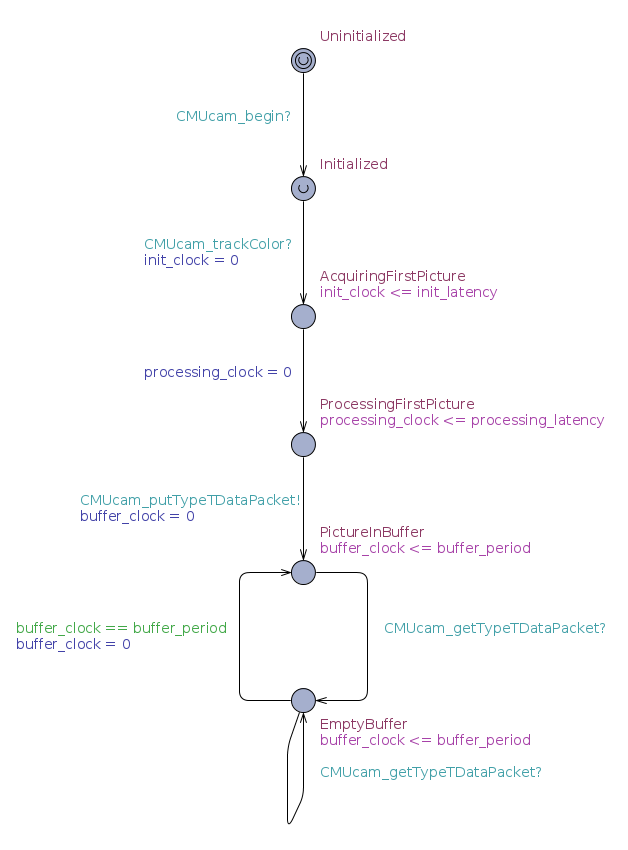
\includegraphics[scale=0.5]{./img/uppaal-camera.png}
      \caption{Modélisation du périphérique {\it Vision Sensor}}
    \end{figure}

    \begin{figure}[!ht]
      \centering
      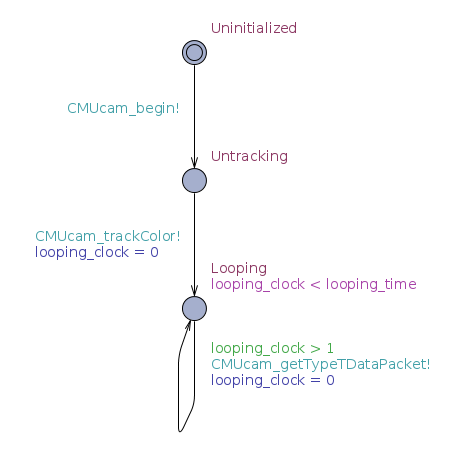
\includegraphics[scale=0.5]{./img/uppaal-loop.png}
      \caption{Modélisation de la tâche {\it Loop}}
    \end{figure}

    \begin{figure}[!ht]
      \centering
      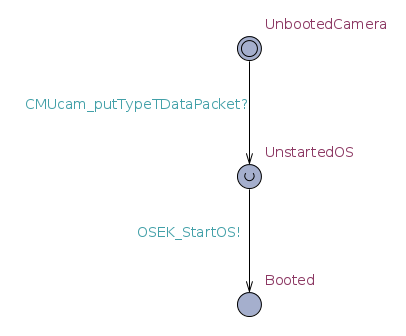
\includegraphics[scale=0.5]{./img/uppaal-boot.png}
      \caption{Modélisation du démarrage du système}
    \end{figure}
    
    \begin{figure}[!ht]
      \centering
      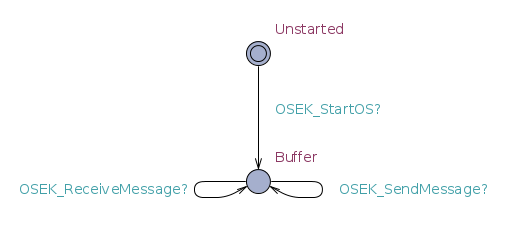
\includegraphics[scale=0.5]{./img/uppaal-buffer.png}
      \caption{Modélisation du buffer du système}
    \end{figure}

    \begin{figure}[!ht]
      \centering
      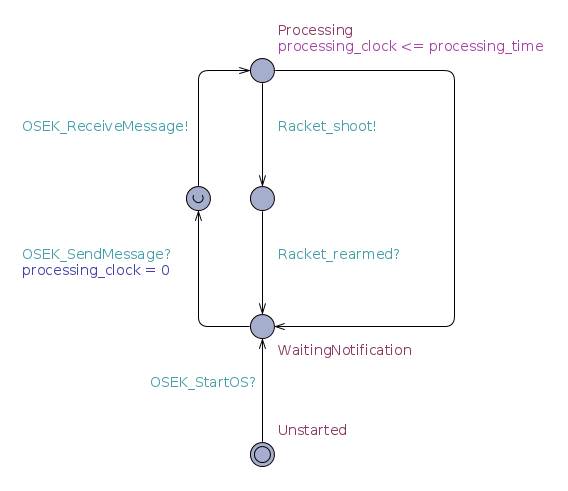
\includegraphics[scale=0.5]{./img/uppaal-task.png}
      \caption{Modélisation de la tâche {\it Control}}
    \end{figure}

    \begin{figure}[!ht]
      \centering
      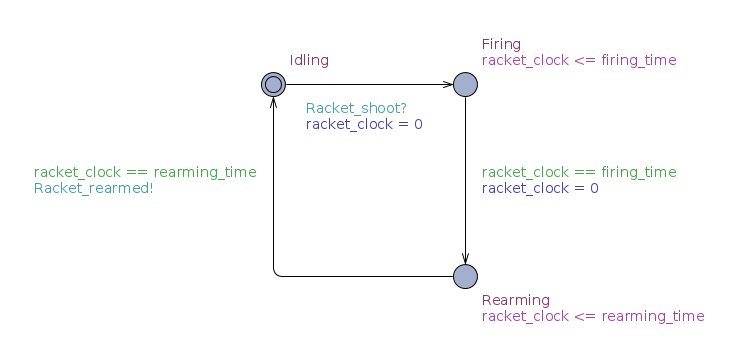
\includegraphics[scale=0.5]{./img/uppaal-racket.png}
      \caption{Modélisation du périphérique {\it Racket}}
    \end{figure}
  
  \FloatBarrier
  \newpage
  \section{Modèle Roméo}
  \label{ann:romeo}

\definecolor{lightgray}{rgb}{.9,.9,.9}

\lstdefinelanguage{cts}{
  keywords={transition, parameters, initially, when, and, do},
  keywordstyle=\bfseries,
  comment=[l]{//},
  commentstyle=\color{purple}
}

\lstset{
  language=cts,
  backgroundcolor=\color{lightgray},
  basicstyle=\footnotesize\ttfamily,
  frame=single,
  rulecolor=\color{black},
  title={Modèle comportemental au format {\it CTS}.}
}

\begin{lstlisting}
  // Declarations:
  parameters 
        init_latency       = 40
    and processing_latency = 60 
    and buffer_period      = 34
    and firing_time        = 5
    and rearming_time      = 7
    and looping_time       = buffer_period
    and polling_time       = 1
    and driver_period      = 50
    and transmission_time  = 2
    and receiving_time     = 4

  initially 
    DEV_camera        := 0,
    DEV_camera_buffer := 0,
    DEV_racket        := 0,
    ARD_loop          := 0,
    ARD_handler       := 0,
    NXT_driver        := 0,
    NXT_driver_period := 0,
    NXT_buffer        := 0,
    NXT_boot          := 0,
    NXT_task          := 0

  // Process DEV_camera:
  transition Camera_Acquiring [0, init_latency]
    when DEV_camera  = 2
    do   DEV_camera := 3

  transition Camera_Updating [buffer_period, buffer_period]
    when DEV_camera  = 4
    do   DEV_camera := 5

  transition Camera_Looping [0, 0]
    when DEV_camera         = 5
    and  DEV_camera_buffer  = 0
    do   DEV_camera        := 4,
         DEV_camera_buffer := 1

  // Process DEV_racket:
  transition Racket_Firing [firing_time, firing_time]
    when DEV_racket  = 1
    do   DEV_racket := 2

  // Processus NXT_driver:
  transition Driver_Activating [driver_period, driver_period]
    when NXT_driver_period  = 1
    do   NXT_driver_period := 0

  // Processus NXT_task:
  transition Task_Processing [0, 0]
    when NXT_task  = 3
    do   NXT_task := 1

  // Synchro CMUcam:
  transition CMUcam_begin
    when ARD_loop    = 0
    and  DEV_camera  = 0
    do   ARD_loop   := 1,
         DEV_camera := 1

  transition CMUcam_trackColor
    when ARD_loop    = 1
    and  DEV_camera  = 1
    do   ARD_loop   := 2,
         DEV_camera := 2

  transition CMUcam_putTypeTDataPacket [0, processing_latency]
    when DEV_camera         = 3
    and  NXT_boot           = 0
    do   DEV_camera        := 4,
         DEV_camera_buffer := 1,
         NXT_boot          := 1

  transition CMUcam_getTypeTDataPacket ]0, looping_time[
    when DEV_camera_buffer  = 1
    and  ARD_loop           = 2
    do   DEV_camera_buffer := 0

  transition CMUcam_getTypeTDataPacket_loop ]0, looping_time[
    when DEV_camera_buffer = 0
    and (DEV_camera = 4 or DEV_camera = 5)
    and  ARD_loop = 2

  // Synchro Driver:
  transition Driver_Busy [0, 0]
    when NXT_driver         = 1
    and  NXT_driver_period  = 0
    and  ARD_handler        = 0
    do   NXT_driver        := 2,
         NXT_driver_period := 1,
         ARD_handler       := 1

  transition Driver_Waiting [receiving_time, receiving_time]
    when NXT_driver   = 4
    and  ARD_handler  = 3
    do   NXT_driver  := 5,
         ARD_handler := 0

  // Synchro Wire:
  transition Wire_onRequest [transmission_time, transmission_time]
    when NXT_driver   = 2
    and  ARD_handler  = 1
    do   NXT_driver  := 3,
         ARD_handler := 2

  transition Wire_write [polling_time, polling_time]
    when ARD_handler  = 2
    and  NXT_driver   = 3
    do   ARD_handler := 3,
         NXT_driver  := 4

  // Synchro OSEK:
  transition OSEK_StartOS [0, 0]
    when NXT_boot    = 1
    and  NXT_buffer  = 0
    and  NXT_driver  = 0
    and  NXT_task    = 0
    do   NXT_boot   := 2,
         NXT_buffer := 1,
         NXT_driver := 1,
         NXT_task   := 1

  transition OSEK_SendMessage [0, 0]
    when NXT_driver  = 5
    and  NXT_buffer  = 1
    and  NXT_task    = 1
    do   NXT_driver := 1,
         NXT_task   := 2

  transition OSEK_ReceiveMessage [0, 0]
    when NXT_task    = 2
    and  NXT_buffer  = 1
    do   NXT_task   := 3

  // Synchro Racket:
  transition Racket_Shoot [0, 0]
    when NXT_task    = 3
    and  DEV_racket  = 0
    do   NXT_task   := 4,
         DEV_racket := 1

  transition Racket_Rearmed [rearming_time, rearming_time]
    when DEV_racket  = 2
    and  NXT_task    = 4
    do   DEV_racket := 0,
         NXT_task   := 1
\end{lstlisting}



\end{document}
